\documentclass[a4paper,11pt,twoside]{tesis}

\usepackage[footnotesize]{caption}

\usepackage[spanish,es-tabla]{babel}
\usepackage[latin1]{inputenc}
\usepackage{etaremune}
\usepackage{hyperref}
\usepackage{dropcaps}
\usepackage{amsfonts,amssymb,amsmath}
\usepackage{latexsym}
\usepackage{makeidx}
\usepackage{epsfig}
\usepackage[mathscr]{eucal}
\usepackage{color}
%\usepackage{macrosangel}
\usepackage[all]{xy}
%\usepackage{macros}
%\usepackage{hyperref}
\usepackage{fancyhdr}
\usepackage{multirow}
\usepackage{cite}
\usepackage{soul}

\usepackage{pdfpages}
\usepackage{appendix}
\usepackage{makeidx}
\usepackage{rotating}


%%%%%%% PAQUETES  ADICIONALES  EN LOS DOS ENTORNO MAC Y PC

%*******   NOTA:   TESIS.STY ha cambiado, he 

\usepackage{programs,keywords}
\usepackage{cancel,calc,underbr}

\usepackage{graphicx}
\usepackage{moreverb}
\usepackage{amssymb,amsmath,color,nicefrac,amsthm}
\usepackage{wasysym}
\usepackage{multicol}
%	\usepackage[latin1]{inputenc}
\usepackage{cancel}
\usepackage{array}
\usepackage[table]{xcolor}
\usepackage{latexsym}

\usepackage{mathrsfs}
%\usepackage[noline,tworuled,figure]{algorithm2e}
\usepackage{url}
\usepackage{pifont}% http://ctan.org/pkg/pifont
\newcommand{\cmark}{\ensuremath{\mathbf\square\!\!\!\!{\checkmark}}}%
\setlength{\leftmargin}{-0.007\textwidth}
\setlength{\textwidth}{1.015\textwidth}
\newcommand{\xmark}{{\ensuremath{\square\!\!\!\!{\times}}}}%
\usepackage[algo2e,ruled,vlined,algochapter,linesnumberedhidden]{algorithm2e}
\usepackage{color}
\newcounter{cpt}
\setcounter{cpt}{1}
\newcommand{\Pcpt}{P\thecpt.\stepcounter{cpt}}

\usepackage{afterpage}

%%%%% PAQUETE PARA COMENTARIOS Y ANOTACIONES

%\usepackage{fixme}
%\fxsetup{
%    status=draft,
%    author= Fernando, % Autor principal del documento
%    layout= margin,
%    theme=color,
%    mode = multiuser % Lo configuramos para edici�n colaborativa
%}
% %\fxuseenvlayout{colorsig}
%
%
% \FXRegisterAuthor{cr}{acr}{Carlos} % registro de autor para Carlos, con los prefijos de los comandos para comentarios y anotaciones
% \FXRegisterAuthor{me}{ame}{Manolo} % registro de autor para Manolo



%%%%%%%%%%%%%%%%%%%%%%%%%%%%%%%%%%%%%%%%%%%%%%%%%%%%%%%%%%%%%%%%%%%%%%%%%%%%%%%%
%%%%%   DEFINITIONS
%%%%%%%%%%%%%%%%%%%%%%%%%%%%%%%%%%%%%%%%%%%%%%%%%%%%%%%%%%%%%%%%%%%%%%%%%%%%%%%%

\newtheorem{theorem}{Teorema}[section]

\newenvironment{notation}
	{\par\smallskip\noindent\textsc{Notation}: }
	{\par\noindent}
\newtheorem{proposicion}[theorem]{Proposici�n}
\newtheorem{definicion}[theorem]{Definici�n}
\newtheorem{ejemplo}[theorem]{Ejemplo}
\newtheorem{corolario}[theorem]{Corolario}
\newtheorem{lema}[theorem]{Lema}
\newtheorem{remark}[theorem]{Nota}
\newtheorem{demostracion}{\textit Demostraci�n}

\def\I{\ensuremath{\mathrel{I}}}
%\bibliographystyle{PhDbiblio-url2} % Title is link if provided
\renewcommand{\bibname}{References} % changes the header; default: Bibliography

\newcommand{\rs}{\textit{sicumaRS}}
\newcommand{\rse}{\textit{sicumaRS} }
%\newcommand{\cierre}{\textit{$Cierre_{SLFD}$}}
%\newcommand{\cierree}{\textit{$Cierre_{SLFD}$} }

% =============== COMANDOS ================
\newcommand{\df}{$R = \langle U,F \rangle$ }
\newcommand{\uno}{$\mathbb{K}$1 }
\newcommand{\dos}{$\mathbb{K}$2 }
\newcommand{\slfd}{$SL_{FD}$}
\newcommand{\slfde}{$SL_{FD}$ }
\newcommand{\sst}{$SST$}
\newcommand{\sste}{$SST$ }
\newcommand{\ssk}{$SSK$} % cierre
\newcommand{\sske}{$SSK$ }
\newcommand{\sck}{$CK$} % cierreIJCM
\newcommand{\scke}{$SCK$ }

\newcommand{\smod}{$SST$}
\newcommand{\smode}{$SST$ }
%\newcommand{\cierre}{$SSK$}
%\newcommand{\cierree}{$SSK$ }
\newcommand{\cierreIJCM}{$SCK$}
\newcommand{\cierreIJCMe}{$SCK$ }
\newcommand{\cierre}{\ref{algoritmo:Cls}}
\newcommand{\cierree}{\ref{algoritmo:Cls} }

\newcommand{\QED}{\hfill {\qed}}


\renewcommand{\appendixname}{Anexo}
\renewcommand{\appendixtocname}{Anexo}
\renewcommand{\appendixpagename}{Anexo}
%
%\renewcommand{\listtablename}{�ndice de tablas} 
%\renewcommand{\tablename}{Tabla} 

%==========================================


% ========================================
% Para no cortar palabras
\hyphenation{na-tu-ra-le-za}
\hyphenation{cir-cuns-tan-cias}
\hyphenation{si-guien-te}
\hyphenation{rea-li-za-do}
\hyphenation{ge-ne-ra-do-res}
\hyphenation{atri-bu-tos}
\hyphenation{re-pre-sen-tar}
\hyphenation{di-fe-ren-tes}
\hyphenation{des-cri-to}
\hyphenation{de-no-mi-na-ron}
\hyphenation{rea-li-zar}
%\hyphenation{ca-rac-te-r�s-ti-cas}
%\hyphenation{je-rar-qu�a}
% ========================================


%----------------------
%    FORMATO DE PAGINA:
%----------------------

\setlength{\evensidemargin}{1cm} \setlength{\oddsidemargin}{2.5cm}
\setlength{\textwidth}{12.5cm} \setlength{\topmargin}{-0.25in}
\setlength{\textheight}{18cm}

\renewcommand{\baselinestretch}{1.15}

\pagestyle{plain}

%\renewcommand{\indexname}{Index}

%---------------------
%       PARA GRAFICOS:
%---------------------

\newdimen\unidad
\unidad = 1mm
\def\caja#1#2{\fbox{\begin{minipage}[t]{#1\unidad} #2 \end{minipage}}}


%\thispagestyle{empty} 
\pagestyle{headings} 
\makeindex



\renewcommand{\theenumi}{\rm(\roman{enumi})}
\renewcommand{\labelenumi}{\theenumi}
\renewcommand{\labelitemi}{\scriptsize $\bullet$}


% ===================================================
\begin{document}
%\renewcommand{\appendixname}{Anexo}
%\renewcommand{\appendixtocname}{Anexo}
%\renewcommand{\appendixpagename}{Anexo}
%
%\renewcommand{\listtablename}{�ndice de tablas} 
%\renewcommand{\tablename}{Tabla} 


\pagestyle{empty}


\frontmatter
\thispagestyle{empty}

\begin{titlepage}

\begin{center}
\vspace*{-1in}
\vspace*{2cm}
\begin{figure}[htb]
\begin{center}
\includegraphics[width=4.5cm]{logoUMAPortada3.jpg}
\end{center}
\end{figure}

Escuela T�cnica Superior de Ingenier�a Inform�tica\\
\vspace*{0.15in}
Departamento de Lenguajes y Ciencias de la Computaci�n \\
\vspace*{0.15in}
Programa de Doctorado en Tecnolog�as Inform�ticas \\

\vspace*{0.4in}

\begin{LARGE}
TESIS DOCTORAL\\
\end{LARGE}

\vspace*{0.2in}

\begin{LARGE}
\textbf{De la Informaci�n al Conocimiento} \\
\end{LARGE}

\vspace*{0.2in}

\begin{Large}
\textbf{Aplicaciones basadas en implicaciones y computaci�n paralela}\\
\end{Large}

\vspace*{0.5in}

\rule{90mm}{0.1mm}\\

\vspace*{0.1in}

\begin{Large}
Autor: D. Fernando Benito Picazo \\
\end{Large}

\vspace*{0.1in}

\begin{large}
Directores: Dr. D. Manuel Nicol�s Enciso Garc�a-Oliveros\\ \ \ \ Dr. D. Carlos Manuel Rossi Jim�nez \\
\end{large}

\vspace*{0.1in}

\begin{large}
M�laga, 2018 \\
\end{large}
\end{center}

\end{titlepage}

% =====================================================================
% =====================================================================
% =====================================================================

\clearemptydoublepage

\newpage{\ } 
\thispagestyle{empty}
\newpage{\ } 
\thispagestyle{empty}

%\include{Portada}
%\clearemptydoublepage

\thispagestyle{empty}

\begin{titlepage}

\begin{center}
\vspace*{-1in}
\vspace*{2cm}
\begin{figure}[htb]
%\begin{center}
%\includegraphics[width=4.5cm]{logoUMAPortada3.jpg}
%\end{center}
\end{figure}

UNIVERSIDAD DE M�LAGA\\
\vspace*{0.20in}
Escuela T�cnica Superior de Ingenier�a Inform�tica\\
\vspace*{0.15in}
Departamento de Lenguajes y Ciencias de la Computaci�n \\
\end{center}
\vspace*{0.15in}

%\vspace*{0.4in}
\noindent
Dr. D. Manuel Nicol�s Garc�a-Oliveros, Catedr�tico de Escuela Universitaria del Departamento de Lenguajes y Ciencias de la Computaci�n de la Universidad de M�laga,\\
Dr. D. Carlos Manuel Rossi Jim�nez, Catedr�tico de Escuela Universitaria del Departamento de Lenguajes y Ciencias de la Computaci�n de la Universidad de M�laga

\vspace*{0.15in}
\noindent
HACEN CONSTAR QUE:
\vspace*{0.150in}

\noindent
D. Fernando Benito Picazo, Ingeniero en Inform�tica, ha realizado en el Departamento de Lenguajes y Ciencias de la Computaci�n de la Universidad de M�laga, bajo nuestra direcci�n, el trabajo de investigaci�n correspondiente a su Tesis Doctoral titulado:

\begin{center}
\begin{LARGE}
De la Informaci�n al Conocimiento \\
\end{LARGE}

\begin{large}
Aplicaciones basadas en implicaciones y computaci�n paralela
\end{large}
\end{center}

\vspace*{0.1in}
\noindent
Revisado el presente trabajo, estimamos que puede ser presentado al tribunal que ha de juzgarlo, y autorizamos la presentaci�n de esta Tesis Doctoral en la
Universidad de M�laga.

\begin{flushright}
M�laga, Noviembre de 2018
\end{flushright}

\vspace*{0.5in}

\begin{center}
Dr. Manuel Nicol�s Garc�a-Oliveros \ \ \ Dr. Carlos Manuel Rossi Jim�nez
\end{center}

\end{titlepage}

% =====================================================================
% =====================================================================
% =====================================================================

\clearemptydoublepage


\thispagestyle{empty}

 
\vspace*{3cm}

\begin{flushright}
\textit{A mi querida Aurora,}
\end{flushright}
 

\begin{flushright}
\textit{a mi padre y a mi madre,}
\end{flushright}

\begin{flushright}
\textit{a mi hermano,}
\end{flushright}
 
\begin{flushright}
\textit{por el apoyo y la confianza que}
\end{flushright}

\begin{flushright}
\textit{siempre me hab�is demostrado.}
\end{flushright}

\vspace*{3cm}

\begin{flushright}
\textit{�Y a la alegr�a de la casa, la Elsita!}
\end{flushright}


\clearemptydoublepage


\vspace*{3cm}

\begin{flushright}
\textit{En todo objetivo conseguido hay siempre una especial tristeza,\\ en el conocimiento de que una meta largamente deseada\\ se ha logrado al fin, y que la vida tiene entonces que ser\\ moldeada y encaminada en busca de nuevos fines.}
\end{flushright}

\begin{flushright}
\textit{La Ciudad y las Estrellas}
\end{flushright}

\begin{flushright}
A. C. Clarke
\end{flushright}

% =====================================================================
% =====================================================================
% =====================================================================

\clearemptydoublepage

\pagestyle{empty}


\setcounter{page}{1}

\selectlanguage{spanish}
\clearemptydoublepage


\chapter*{Agradecimientos}\label{agradecimientos_chapter}  
%\addcontentsline{toc}{chapter}{\protect{Agradecimientos}}
\thispagestyle{empty}
\markboth{Agradecimientos}{Agradecimientos}
%Agradecimientos
%
%dadsadsad
%
%as
%dasdas
%d
%sa
%dsad
%
%
%
%sd
%as
%dsa
%d
%
%
%
%adsasda

%



\noindent
A menudo he escuchado que esta es la parte que m�s dif�cil resulta redactar; coincido con ello, pero tambi�n tengo claro que es la que m�s he disfrutado escribiendo. 

\vspace{0.3cm}

Ahora que ya se termina esta etapa de mi vida con la consecuci�n de esta tesis doctoral, es momento de hacer balance y de agradecer a las personas que han intervenido en este gran logro; porque es tambi�n gracias a ellos.

En primer lugar, quiero agradecer a mis queridos directores, Dr. Manuel Enciso y Dr. Carlos Rossi, la direcci�n de la tesis y todo lo que me hab�is ense�ado, pero en especial, vuestro trato, con el que siempre me hab�is hecho sentir uno de vosotros, y donde la acogida siempre ha sido la mejor; por todo ello, gracias.

Manolo, me has dirigido: el proyecto fin de carrera de la ingenier�a t�cnica de sistemas, el proyecto fin de carrera de la ingenier�a superior, el trabajo fin de m�ster, y ahora, la tesis doctoral. Quiero decirte que me siento orgulloso de ello, y que si tuviera que volver a recorrer todo ese camino, volver�a a pedirte que estuvieras de nuevo a mi lado; por todo ello, gracias.

Carlos, lo primero es decirte que ojal� nos hubi�ramos cruzado antes. Adem�s de por la direcci�n de la tesis, tambi�n quiero darte las gracias por haber buscado siempre posibilidad de financiaci�n para que pudiera afrontar este periodo de investigaci�n con un respaldo; por todo ello, gracias.

Quiero hacer menci�n especial al Dr. Sergio G�lvez. Sergio, ha sido una gran suerte tenerte cerca para dudas y consejos, y en realidad, por el simple hecho de conversar contigo. Siempre me has apoyado y valorado mucho, y eso significa mucho para m�; por todo ello, gracias.

Gracias a mis coautores: Dr. Pablo Cordero, Dr. �ngel Mora, Dr. Antonio Guevara, ha sido un placer publicar a vuestro lado; a la Dra. Llanos Mora como tutora de tesis; al Dr. Antonio Vallecillo por buscar un contacto en el momento preciso; al Dr. Dar�o Guerrero y al Dr. Rafael Larrosa por el apoyo en el Centro de Supercomputaci�n.

Ahora, quiero darte las gracias a ti, mi querida Aurora, por ser mi apoyo y �nimo diario e incondicional, por quererme siempre cada d�a y soportar mi insaciable inquietud, y por haber vivido juntos todos estos �xitos que la vida nos est� deparando, que seguro, a tu lado, ser�n muchos m�s.

Lo primero que quiero decirle a mi padre y a mi madre es: lo he conseguido. Gracias por darme el mejor entorno familiar posible, por vuestro interminable esfuerzo y por inculcarme la vital importancia de la educaci�n y el saber. Ahora es momento de recoger los frutos y disfrutar de lo que hemos conseguido todos juntos. 

Gracias tambi�n a ti, hermano, por ser la persona que m�s me ha ense�ado en la vida y de quien sigo aprendiendo a cada momento juntos. Gracias por estar siempre disponible y por encauzarme y guiarme por el infinito camino de la Ciencia.

Quiero hacer un gui�o a mis profesores de la ni�ez, D. Justo, D. Juli�n, D. Luis y D. Andr�s, por construir a tan temprana edad, unos s�lidos cimientos sobre los que crecer.

Seguramente olvide alguien, no obstante, gracias a toda persona que hasta el d�a de hoy me haya ense�ado cualquier cosa, pues para m�, lo m�s importante es el Conocimiento.


% =====================================================================
% =====================================================================
% =====================================================================
\clearemptydoublepage

%\selectlanguage{english}

\pagestyle{headings}



%===============================================================
%           Fin  Agradecimiento
%===============================================================



\tableofcontents 
\clearemptydoublepage

\selectlanguage{spanish}


%\selectlanguage{english}
\chapter*{Publicaciones}
\label{cap:publicaciones}
\addcontentsline{toc}{chapter}{\protect{Publicaciones}}

\markboth{Publicaciones}{Publicaciones}

A continuaci�n se expone una lista de los trabajos que han sido publicados como resultado de la investigaci�n llevada a cabo a lo largo de esta tesis doctoral. Estas publicaciones avalan el trabajo realizado poniendo de manifiesto tanto su inter�s como su validez cient�fica.\\

\begin{Large}
Revistas
\end{Large}

\begin{enumerate}
	\item Fernando Benito-Picazo, Pablo Cordero, Manuel Enciso, �ngel Mora. \textit{Minimal generators, an affordable approach by means of massive computation}. The Journal of Supercomputing, Springer, 2018. 
	
	{\tt DOI: 10.1007/s11227-018-2453-z}
	
Factor de impacto en J.C.R. 2017: 1,532. Posici�n 43 de 103 (Q2) en la categor�a: `Computer Science, Theory \& Methods'.
	\item Fernando Benito-Picazo, Manuel Enciso, Carlos Rossi, Antonio Guevara. \textit{Enhancing the conversational process by using a logical closure operator in phenotypes implications}. Mathematical Methods in the Applied Sciences, John Wiley \& Sons Ltd, 2017. 
	
	{\tt DOI: 10.1002/mma.4338}
	
Factor de impacto en J.C.R. 2017: 1,18. Posici�n 91 de 252 (Q2) en la categor�a: `Mathematics, Applied'.
	\item Fernando Benito-Picazo, Pablo Cordero, Manuel Enciso, �ngel Mora. \textit{Reducing the search space by closure and simplification paradigms. A parallel key finding method}. The Journal of Supercomputing, Springer, 2016. 
	
	{\tt DOI: 10.1007/s11227-016-1622-1}
	
Factor de impacto en J.C.R. 2016: 1,349. Posici�n 52 de 104 (Q2) en la categor�a: `Computer Science, Theory \& Methods'.
\end{enumerate}

\begin{Large}
Congresos Internacionales
\end{Large}

\begin{itemize}
	\item Fernando Benito-Picazo, Pablo Cordero, Manuel Enciso, �ngel Mora. \textit{Closed sets enumeration: a logical approach}. Proceedings of the Seventeenth International Conference on Computational and Mathematical Methods in Science and Engineering, CMMSE, 2017. C�diz, Spain, July 4-8, pp. 287-292, ISBN: 978-84-617-8694-7.
	\item Fernando Benito-Picazo, Manuel Enciso, Carlos Rossi, Antonio Guevara. \textit{Conversational recommendation to avoid the cold-start problem}. Proceedings of the Sixteenth International Conference on Computational and Mathematical Methods in Science and Engineering, CMMSE, 2016. C�diz, Spain, July 4-8, pp. 184-190, ISBN: 978-84-608-6082-2.
	\item Fernando Benito-Picazo, Pablo Cordero, Manuel Enciso, �ngel Mora. \textit{Keys for the fusion of heterogeneous information}. Proceedings of the Fifteenth International Conference on Computational and Mathematical Methods in Science and Engineering, CMMSE, 2015. C�diz, Spain, July 6-10, pp. 201-211, ISBN: 978-84-617-2230-3.
	\item Fernando Benito-Picazo, Pablo Cordero, Manuel Enciso, �ngel Mora. \textit{Increasing the Efficiency of Minimal Key Enumeration Methods by Means of Parallelism}. Proceedings of the 9th International Conference on Software Engineering and Applications, ICSOFT-EA, Vienna, Austria, August 29-31, 2014, pp. 512-517.
	
	{\tt DOI: 10.5220/0005108205120517} 
\end{itemize}

\newpage
\begin{Large}
Workshops
\end{Large}

\begin{itemize}
	\item Fernando Benito-Picazo. \textit{Parallelism in the search of minimal keys from implications using tableaux methods}. Workshop: L�gica, Lenguaje e Informaci�n. Dpto. Matem�tica Aplicada. Unidad de Investigaci�n en L�gica, Lenguaje e Informaci�n, Andaluc�a Tech. Universidad de M�laga, Noviembre 2014.
\end{itemize}

\vspace{0.5cm}

\begin{figure}[htbp]
		\begin{center}
			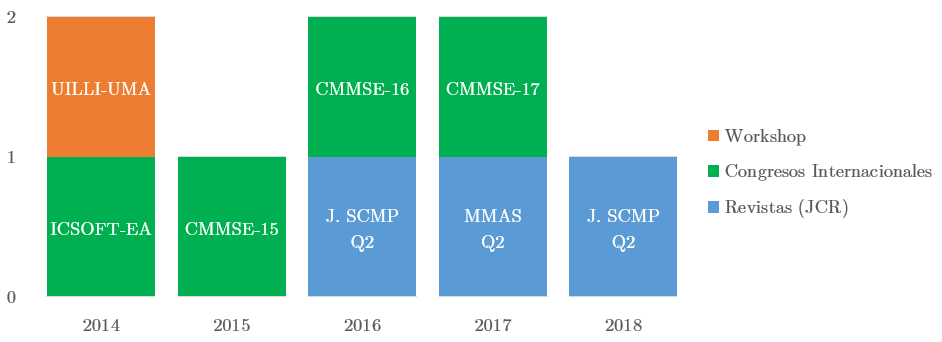
\includegraphics[height=.23\textheight,width=.95\textwidth]{graficoPublicaciones.png}
		\end{center}
		\caption{Producci�n cient�fica}
		\label{figura:graficoPublicaciones}
\end{figure}



% =====================================================================
% =====================================================================
% =====================================================================
\clearemptydoublepage


%\include{resumen}
%\clearemptydoublepage

%\include{overview}
%\clearemptydoublepage

\pagestyle{headings}

%%%%%%%%%%%%%%%%%%%%%% OBJETIVOS, APORTACIONES Y ESTRUCTURA

%%%%%%%%%%%%%%%%%%%%%% PRELIMINARES algebraicos

\selectlanguage{spanish}

\mainmatter

\pagestyle{empty}
\chapter{Introducci�n}\label{cap:introduccion}
%\epigraphfontsize{\small\itshape}
\setlength{\epigraphwidth}{8.7cm}
\epigraph{\textit{---Empieza por el principio ---dijo el Rey con gravedad--- y sigue hasta llegar al final; all�, te paras.
}{\\\textit{\ \ \ \ \ \ \ \ \ \ \ \ \ \ \ \ \ \ \ \ \ \ \ \ \ \ \ \ Alicia en el pa�s de las maravillas}\\\textup{\ \ \ \ \ \ \ \ \ \ \ \ \ \ \ \ \ \ \ \ \ \ \ \ \ \ \ \ \ \ \ \ \ \ \ \ \ \ \ \ \ \ \ \ \ \ \ \ \ \ \ \ \ \ \ \ \ \ \ \ \ \ L. Carroll}}
}

\pagestyle{headings}

\bigdrop{0pt}{5}{cmr10}La gesti�n de la informaci�n es uno de los pilares esenciales de la Ingenier�a Inform�tica. No es de extra�ar, por tanto, que conforme un amplio campo de investigaci�n y conocimiento donde diversas disciplinas como las Matem�ticas, la L�gica y la Computaci�n act�en conjuntamente para alcanzar mejores sinergias.

Dentro de este �mbito y con la intenci�n de hacer aportaciones en campos de la Ingenier�a Inform�tica como son las bases de datos\index{bases de datos} y los sistemas de recomendaci�n\index{sistemas de recomendaci�n}, esta tesis doctoral toma como principal base te�rica el An�lisis Formal de Conceptos \index{An�lisis Formal de Conceptos} (FCA, por sus siglas en ingl�s: \textit{Formal Concept Analysis}), y m�s concretamente, una de sus herramientas fundamentales: los conjuntos de implicaciones\index{conjuntos de implicaciones}. La gesti�n inteligente de estos elementos mediante t�cnicas l�gicas y computacionales confieren una alternativa para superar obst�culos en los campos mencionados.

FCA es una teor�a matem�tica y una metodolog�a que permite derivar una jerarqu�a de conceptos a partir de una colecci�n de objetos, sus atributos y las relaciones entre ellos. De esta forma, el prop�sito es poder representar y organizar la informaci�n de manera m�s cercana al pensamiento humano sin perder rigor cient�fico. En este sentido se enmarca la cita de Rudolf Wille: ``\textit{El objetivo y el significado del FCA como teor�a matem�tica sobre conceptos y sus jerarqu�as es apoyar la comunicaci�n racional entre seres humanos mediante el desarrollo matem�tico de estructuras conceptuales apropiadas que se puedan manipular con la l�gica.}'' \cite{Wille2005}.

El t�rmino FCA fue acu�ado por Wille en 1984 culminando a�os m�s tarde con la publicaci�n m�s citada al respecto en colaboraci�n con Bernhard Ganter \cite{Ganter1997}. Desde entonces, FCA se ha aplicado con �xito en diferentes disciplinas, como por ejemplo: biolog�a celular \cite{Endres2012}, gen�tica \cite{Xudong2015}, ingenier�a del software \cite{Poelmans2012,Kester2013}, medicina \cite{Sacarea2017}, derecho \cite{Mimouni2015}, etc.

FCA parte de una representaci�n de conjuntos de objetos y atributos por medio de tablas de datos. Estas tablas se denominan contextos formales y representan las relaciones binarias entre esos objetos y atributos. A partir de ah�, se generan dos herramientas b�sicas para representar el conocimiento: los ret�culos de conceptos y los conjuntos de implicaciones. Dichas herramientas adem�s, son representaciones equivalentes del conocimiento descrito en el contexto formal.

Desde hace a�os, existen en la literatura estudios \cite{Kuznetsov2002,Outrata2012} donde se han investigado y comparado diferentes algoritmos para obtener el ret�culo de conceptos a partir de un conjunto de datos (en adelante \textit{dataset} por su nomenclatura habitual en el campo)\index{dataset}. Muchos de ellos toman como base uno de los algoritmos m�s conocidos a tal efecto, el denominado por Wille y Ganter como \textit{NextClosure} \cite{Ganter1997}.
%Sin embargo, debido a que el tama�o del ret�culo de conceptos es, en el peor de los casos, $2^{min(|G|,|M|)}$, siendo $G$ el conjunto de objetos y $M$ el conjunto de atributos, el coste computacional de los m�todos encargados de su construcci�n constituye una limitaci�n para la aplicaci�n de FCA.

Por otro lado est� el conjunto de implicaciones. Las implicaciones pueden considerarse \textit{grosso modo} como reglas del tipo \textit{si-entonces}, que representan un concepto muy intuitivo: cuando se verifica una premisa, entonces se cumple una conclusi�n. Esta idea b�sica se utiliza con diferentes interpretaciones en numerosos campos de conocimiento. As�, en la teor�a relacional se interpretan como dependencias funcionales (DFs)\index{dependencias funcionales} \cite{Codd1971b}, en FCA como implicaciones\index{implicaciones} \cite{Ganter1997}, etc�tera.

No obstante, tambi�n existen ciertas desventajas a la hora de trabajar con ret�culos e implicaciones, de hecho, la propia extracci�n del conjunto completo de implicaciones de un \textit{dataset} es una tarea que presenta una complejidad exponencial, sin embargo, es conveniente destacar que no es competencia de este trabajo el estudio de t�cnicas de extracci�n de implicaciones (lo cual es m�s una tarea de miner�a de datos), sino que la intenci�n es partir del conjunto de implicaciones para trabajar con �l. A este respecto, se pueden consultar trabajos ampliamente citados en la literatura en relaci�n a la extracci�n de implicaciones a partir de \textit{datasets}\index{dataset} \cite{HuhtalaKPT99,YaoHB2002}.

Trabajar con conjuntos de implicaciones permite utilizar t�cnicas de razonamiento autom�tico basadas en la l�gica. Este hecho fundamenta el objetivo de esta tesis doctoral, que principalmente consiste en, utilizando los conjuntos de implicaciones, aplicar mecanismos l�gicos para realizar un tratamiento eficiente de la informaci�n.

Como se ver� en el Cap�tulo \ref{cap:preliminares}, la aproximaci�n a trav�s de la l�gica es posible gracias a sistemas axiom�ticos correctos y completos como los axiomas de Armstrong\index{Axiomas de Armstrong} \cite{Armstrong74} y la L�gica de Simplificaci�n\index{L�gica de Simplificaci�n} \cite{Enciso2002} (SL, por sus siglas en ingl�s: \textit{Simplification Logic}). Estos m�todos aplicados sobre conjuntos de implicaciones se utilizan en esta tesis doctoral sobre tres �reas de investigaci�n: claves minimales\index{clave!claves minimales}, generadores minimales\index{generadores minimales} y sistemas de recomendaci�n conversacionales.

Se anticipa que, en cada uno de los casos, se va a aprovechar la informaci�n subyacente al conjunto de implicaciones para realizar novedosas aproximaciones que permitan abordar problemas presentes en esos �mbitos. Los resultados obtenidos se sustentan por una amplia gama de experimentos, en los cuales se ha utilizado tanto informaci�n real como sint�tica (informaci�n generada de forma aleatoria) y donde la computaci�n paralela llevada a cabo en entornos de supercomputaci�n\index{supercomputaci�n} ha desempe�ado un papel crucial. Como se ver� m�s adelante, para el primer caso, el trabajo se centra en el uso de DFs mientras que para el segundo y tercero el n�cleo son implicaciones.

%Antes de describir con mayor detalle las tres �reas anteriores, es necesario hacer una importante declaraci�n previa. Tal y como se ha mencionado anteriormente, en esta tesis se trabaja con el conjunto de implicaciones que se deriva de un \textit{dataset}.  

%Son trabajos de suma importancia desde el punto de vista te�rico, pero tambi�n desde el punto de visto pr�ctico, pues incluyen las implementaciones de las aplicaciones que realizan la extracci�n de las implicaciones. 

Dicho esto, se retoma el texto pasando a introducir los tres campos de aplicaci�n donde se han utilizado los conjuntos de implicaciones.

%Sin perjuicio de lo anterior, dado que hemos llegado a crear datasets propios sobre los que poder realizar experimentos como veremos m�s adelante, si bien no entramos en las t�cnicas de extracci�n de implicaciones que utilizan esas aplicaciones, s� hemos tenido que convertirnos en usuarios de estas aplicaciones para poder obtener el conjunto atributos e implicaciones que se verifican. Dicho esto, retomamos el texto pasando a introducir los tres campos de aplicaci�n donde hemos utilizado los conjuntos de implicaciones.

\section{Claves Minimales}
\noindent
El concepto de clave\index{clave} es fundamental en cualquier modelo de datos, incluyendo el modelo de datos relacional de Codd \cite{Codd1990}. Una clave de un esquema relacional est� compuesta por un subconjunto de atributos\index{atributo} que identifican a cada uno de los elementos de una relaci�n. Representan el \textit{dominio} de una determinada funci�n cuya \textit{imagen} es la totalidad del conjunto de atributos. As�, en un esquema de bases de datos relacional, una clave permite identificar cada fila de una tabla, impidiendo que exista m�s de una fila con la misma informaci�n y puede representarse por medio de una DF \cite{Codd1990} hacia todo el conjunto de atributos. Debido a ello en los sistemas gestores de bases de datos, las restricciones de clave son implementadas usando restricciones de unicidad (\textit{unique}) sobre el subconjunto de atributos que forman la clave.

Las DFs especifican una relaci�n entre dos subconjuntos de atributos, e.g. $A$ y $B$, representada como $A \to B$, que asegura que para cualesquiera dos tuplas\index{tupla} de una tabla de datos, si los valores de sus atributos de $A$ coinciden, entonces tambi�n han de coincidir los de $B$. Si bien la noci�n de DF se ver� con mayor detalle en la Secci�n \ref{sec:basesDatosRelacionales}, se adelanta el siguiente ejemplo b�sico \ref{ejemplo:basicoClaves} tanto para mostrar ejemplos de DFs como para ilustrar el concepto de clave.

\begin{ejemplo}
\label{ejemplo:basicoClaves}
Supongamos que disponemos de la siguiente tabla con informaci�n que relaciona t�tulos de pel�culas, actores, pa�ses, directores, nacionalidad y a�os de estreno:

\vspace{0.3cm}
\noindent
{\scriptsize
\begin{tabular}{lcllll}
 \hline
 T�tulo & A�o & Pa�s & Director & Nacionalidad & Actor\\
 \hline
 Pulp Fiction & 1994 & USA & Quentin Tarantino & USA & John Travolta\\
 Pulp Fiction & 1994 & USA & Quentin Tarantino & USA & Uma Thurman\\
  Pulp Fiction & 1994 & USA & Quentin Tarantino & USA &Samuel Jackson \\
 King Kong & 2005 & NZ & Peter Jackson& NZ & Naomi Watts\\
 King Kong & 2005 & NZ & Peter Jackson & NZ & Jack Black\\
 King Kong & 1976 & USA & De Laurentiis & IT & Jessica Lange\\
 King Kong & 1976 & USA & De Laurentiis & IT & Jeff Bridges\\
 Django Unchained & 2012 & USA & Quentin Tarantino  & USA & Jamie Foxx\\
 Django Unchained & 2012 & USA & Quentin Tarantino  & USA & Samuel Jackson\\
 Blade Runner & 1982 & USA & Ridley Scott & UK & Harrison Ford\\
 Blade Runner & 2017 & USA & Denis Villeneuve  & CAN & Harrison Ford\\
% El dictador & 2012 & USA & Larry Charles  & USA & Megan Fox\\
% This is 40 & 2012 & USA & Judd Apatow  & USA & Megan Fox\\
 \hline
\end{tabular}
}

\vspace{0.3cm}

De esta informaci�n, podemos extraer el siguiente conjunto de DFs: 

$\Sigma = \{Titulo, A\tilde{n}o \rightarrow Pais, Director$; $Director\rightarrow Nacionalidad$\}. 

Esta tabla tiene una �nica clave: $\{A\tilde{n}o, Actor\}$ que corresponde con el conjunto de atributos necesario para identificar cualquier tupla de la relaci�n.
\end{ejemplo}

La identificaci�n de las claves de una determinada relaci�n es una tarea crucial para muchas �reas de tratamiento de la informaci�n: modelos de datos \cite{Simsion2005}, optimizaci�n de consultas \cite{Kemper1991}, indexado \cite{Manolopoulos1999}, enlazado de datos \cite{Nikolov2011}, etc. Como muestras de esta importancia, es posible encontrar numerosas citas en la literatura, entre las que se pueden destacar las siguientes. En \cite{Sismanis2006}, los autores afirman que: ``\textit{la identificaci�n de claves es una tarea fundamental en muchas �reas de la gesti�n moderna de datos, incluyendo modelado de datos, optimizaci�n de consultas (proporciona un optimizador de consultas con nuevas rutas de acceso que pueden conducir a mejoras sustanciales en el procesado de consultas), indexaci�n (permite al administrador de la base de datos mejorar la eficiencia del acceso a los datos a trav�s de t�cnicas como la partici�n de datos o la creaci�n de �ndices y vistas), detecci�n de anomal�as e integraci�n de datos}''. En \cite{Pernelle2013} los autores delimitan el problema manifestando: \textit{``establecer enlaces sem�nticos entre los elementos de datos puede ser realmente �til, ya que permite a los rastreadores, navegadores y aplicaciones combinar informaci�n de diferentes fuentes.''}.

Como refleja el contenido de esta secci�n, es evidente la importancia manifiesta de averiguar las claves de una relaci�n, sin embargo, este labor no est� exenta de dificultades, por ello, el trabajo realizado en esta parte de la tesis ha consistido en proponer, dise�ar e implementar m�todos para afrontar el problema de la b�squeda de claves, el cual se presenta a continuaci�n.


% El problema de la b�squeda de claves
\section*{El Problema de la B�squeda de Claves}
\label{sec:problemaBusquedaClaves}
\noindent
% Problema de la b�squeda de claves
El problema de la b�squeda de claves consiste en encontrar todos los subconjuntos de atributos que componen una clave minimal\footnote{Se acu�a el t�rmino \textit{minimal} para referirnos a una clave en la que todos y cada uno de los atributos que la forman son imprescindibles para mantener su naturaleza de clave, es decir, no contiene ning�n atributo superfluo.} a partir de un conjunto de DFs. Es un campo de estudio con d�cadas de antig�edad como puede observarse en \cite{Sali2004}, o en \cite{Fadous75}, donde las claves se estudiaron dentro del �mbito de la matriz de implicaciones.

% Claves como elemento crucial
%La dificultad al enfrentarse al problema de la b�squeda de claves surge debido a que, dado un conjunto de atributos $A$, la cardinalidad del conjunto $2^A$ hace que haya que abordar el problema aplicando t�cnicas que gu�en la b�squeda de los conjuntos candidatos a ser claves minimales de forma que se pueda subsanar la complejidad exponencial de este tipo de problemas. 

% problema NP
El c�lculo de todas las claves minimales representa un problema complejo. En \cite{Lucchesi78,Yu76} se incluyen resultados interesantes acerca de la complejidad del problema; los autores demuestran que el n�mero de claves est� limitado por el factorial del n�mero de dependencias, por tanto, no existe un algoritmo que resuelva el problema en tiempo polin�mico. En definitiva, es un problema NP-completo decidir si existe una clave de tama�o a lo sumo $k$ dado un conjunto de DFs.

Por otro lado, en \cite{CorderoEMG14}, los autores muestran c�mo el problema de las claves minimales en las bases de datos tiene su an�logo en FCA, donde el papel de las DFs se trata como implicaciones de atributos. En ese art�culo, el problema de las claves m�nimales se present� desde un punto de vista l�gico y para ello, se emple� un sistema axiom�tico, que los autores denominaron \slfde\index{\slfde} (por sus siglas en ingl�s: \textit{Simplification Logic for Functional Dependencies}) \cite{Enciso2002}, para gestionar las DFs y las implicaciones.

% referencias generales
Las principales referencias sobre el problema de la b�squeda de claves apuntan al trabajo de Lucchesi y Osborn en \cite{Lucchesi78} donde presentan un algoritmo para calcular todas las claves. Por otro lado, Saiedian y Spencer \cite{Saiedian1996} presentaron un algoritmo usando grafos con atributos para encontrar todas las claves posibles de un esquema de base de datos relacional. No obstante, demostraron que s�lo pod�a aplicarse cuando el grafo de DFs no estuviera fuertemente conectado. Es rese�able tambi�n el trabajo de Zhang \cite{Zhang09} en el cual se utilizan mapas de Karnaugh \cite{Karnaugh1953} para calcular todas las claves. Existen  m�s trabajos sobre el problema del c�lculo de las claves minimales como son \cite{Sismanis2006,Worland2004}. %Asimismo, en \cite{Levy2005,Valtchev03,Valtchev08} los autores propusieron el uso de FCA \cite{Ganter1997} para abordar problemas relacionados con la b�squeda y la gesti�n de las implicaciones, que pueden considerarse complementarios a nuestro trabajo.




\section*{Algoritmos para el C�lculo de Claves}
\label{sec:algoritmosCalculoClaves}
\noindent
% referencias de tableaux
El objetivo de esta parte de la tesis se centra en los algoritmos de b�squeda de claves basados en la l�gica, y m�s espec�ficamente, en aquellos que utilizan el paradigma de tableaux\index{Tableaux} \cite{Morgan1992,Risch1992} como sistema de inferencia. 

De forma muy general, se puede decir que los m�todos tipo tableaux representan el espacio de b�squeda como un �rbol, donde sus hojas contienen las soluciones (claves). El proceso de construcci�n del �rbol comienza con una ra�z inicial y desde all�, mediante la utilizaci�n de unas reglas de inferencia, se generan nuevas ramas del �rbol etiquetadas con nodos que representan instancias m�s simples del nodo padre. Debido a esta caracter�stica, las comparaciones entre estos m�todos se pueden realizar f�cilmente ya que su eficiencia va de la mano del tama�o del �rbol de b�squeda generado. La mayor ventaja de este proceso es su versatilidad, ya que el desarrollo de nuevos m�todos se reduce en gran parte a cambiar las reglas de inferencia.

Esto conduce a un punto de partida fundamental, los estudios de R. Wastl (Universidad de Wurzburg, Alemania) \cite{Wastl98a,Wastl98} donde se introduce por primera vez un sistema de inferencia de tipo Hilbert para averiguar todas las claves de un esquema relacional. %A modo de ejemplo b�sico, en la Figura \ref{figura:ejemploTaleaux} se presenta un �rbol de b�squeda seg�n el paradigma de tableaux desarrollado utilizando el sistema de inferencia $\mathbb{K}$ de Wastl. 
B�sicamente, se parte de una ra�z para cuyo c�lculo se ha aplicado una regla de inferencia \uno y a partir de ah�, se van construyendo las diferentes ramas del �rbol mediante la aplicaci�n de una segunda regla de inferencia \dos al conjunto de DFs (v�ase \cite{Wastl98a,Wastl98} para m�s detalles).

%\begin{figure}[htbp]
%	\begin{center}
%		\includegraphics*[width=.75\textwidth,height=.25\textheight]{arbol897.png}
%	\end{center}
%	\caption{Ejemplo de tableaux utilizando el sistema de inferencia $\mathbb{K}$ de Wastl.}
%	\label{figura:ejemploTaleaux}
%\end{figure}

%\begin{figure}[htbp]
%	\begin{center}
%\begin{tikzpicture}%[every node/.style={rectangle, fill=blue!20!white}]
%\node {ABCD} [sibling distance=2.5cm]
%child {node {BCD}
%child {node {BC}}
%}
%child {node {ACD}
%child {node {CD}}
%}
%child {node {BCD}
%child {node {BC}}
%}
%child {node {ABC}
%child {node {BC}}
%child {node {AC}}
%};
%\end{tikzpicture}
%\end{center}
%\caption{Ejemplo de tableaux utilizando el sistema de inferencia $\mathbb{K}$ de Wastl.}
%\label{figura:ejemploTaleaux}
%\end{figure}

Siguiendo esta l�nea, en \cite{Cordero2013} los autores abordan el problema de la b�squeda de claves utilizando un sistema de inferencia basado en la l�gica \slfde \cite{Enciso2002}, demostrando como el �rbol del espacio de b�squeda que se genera lleva a sobrepasar las capacidades computacionales de ordenadores corrientes hoy d�a, incluso para problemas peque�os. En \cite{Enciso2002} los autores muestran la equivalencia entre \slfde\index{\slfde} y los axiomas de Armstrong \cite{Armstrong74} junto con un algoritmo para calcular el cierre de un conjunto de atributos. M�s tarde, en \cite{CorderoEMG14}, los autores introdujeron el m�todo SST (por sus siglas en ingl�s, \textit{Strong Simplification Tableaux})\index{SST} para calcular todas las claves minimales usando una estrategia de estilo tableaux, abriendo la puerta a incorporar el paralelismo en su implementaci�n. 

El m�todo SST est� basado en la l�gica de simplificaci�n y sus equivalencias, a�adiendo adem�s, el test de minimalidad para aumentar la eficiencia. De esta forma, SST evita la apertura de ramas adicionales del �rbol, por lo que el espacio de b�squeda se vuelve m�s reducido, logrando un gran rendimiento en comparaci�n con sus predecesores como puede comprobarse en el amplio estudio realizado sobre el m�todo en \cite{Benito-Picazo2014TFM}.


%\section*{M�todos \textit{SST} y \textit{CK}}
%\label{sec:metodosSSTyCK}
%\noindent
%En \cite{CorderoEMG14} se present� un nuevo algoritmo, denominado SST\index{SST}, para calcular todas las claves minimales usando una estrategia de estilo tableaux, abriendo la puerta a incorporar el paralelismo en su implementaci�n. SST se basa en la noci�n de cierre de conjunto; una noci�n b�sica en la teor�a de bases de datos que, utilizando el sistema axiom�tico\index{sistema axiom�tico} de la l�gica \slfde (ver Secci�n \ref{subsec:logicaSLFD}), permite caracterizar el conjunto m�ximo de atributos que se puede alcanzar, desde un determinado conjunto de atributos $A$ con respecto a un conjunto de DFs. Por lo tanto, si el cierre de $A$ se denota como $A^+_\Sigma$, el sistema de inferencia para DFs permite inferir la DF $A\to A^+_\Sigma$. En este sentido, el enfoque con estilo l�gico para el problema de las claves minimales consiste en la enumeraci�n de todos los conjuntos de atributos $A$ tales que se verifique la DF: $A\to M$.

%SST muestra un gran rendimiento en comparaci�n con sus predecesores como puede comprobarse en el amplio estudio realizado sobre el m�todo en \cite{Benito-Picazo2014TFM}. El beneficio principal en la reducci�n del espacio de b�squeda se debe a la introducci�n de un test de inclusi�n para evitar la apertura de la totalidad de las ramas del �rbol. Gracias a ello, SST no abre aquellas ramas de las que se tiene el conocimiento de que van a producir las mismas claves que se calculan en otra rama.

Por otro lado, el nuevo operador de cierre\index{operador de cierre} definido en \cite{Mora2012} tiene una caracter�stica fundamental que lo convierte en una novedosa alternativa frente a los m�todos cl�sicos \cite{Maier1983} y es la siguiente. Adem�s del conjunto de atributos que se deriva de la aplicaci�n del operador de cierre al conjunto de implicaciones, el m�todo proporciona un subconjunto $\Sigma^\prime$ de implicaciones del conjunto $\Sigma$ original que engloba la informaci�n que ha quedado fuera del cierre.

Tomando como base esos trabajos anteriores y con el apoyo del sistema axi�matico de la l�gica \slfde\index{\slfde} (v�ase Secci�n \ref{subsec:logicaSLFD}), en esta tesis se presenta un nuevo m�todo llamado \textit{Closure Keys (CK)}\index{CK}. Este nuevo m�todo incorpora un mecanismo eficiente de poda que utiliza el m�todo de cierre basado en \slfde (ver Secci�n \ref{subsec:algoritmosCalculoCierre}) para mejorar el rendimiento del m�todo SST. 

%El m�todo CK tiene una caracter�stica fundamental que lo convierte en una novedosa alternativa frente a los m�todos cl�sicos y es la siguiente. Adem�s del conjunto de atributos que se deriva de la aplicaci�n del operador de cierre al conjunto de implicaciones, el m�todo proporciona un subconjunto $\Sigma$ de implicaciones del conjunto $\Sigma$ original que engloba la informaci�n que ha quedado fuera del cierre. 

%M�s formalmente, el m�todo CK recibe un conjunto de implicaciones $\Sigma$ y un subconjunto de atributos $X \subseteq \Omega$, calcula el conjunto cierre $X^+$ respecto a $\Sigma$, y adem�s, un nuevo conjunto $\Sigma$ que contiene el conjunto de implicaciones que guarda la sem�ntica que queda fuera del cierre $X^+$. Si $\Sigma = \varnothing$, entonces $X^+ = \Omega$ (v�ase \cite{Mora2012} para m�s detalles).
%Con esto, se tienen los elementos para presentar la principal contribuci�n de la tesis en la resoluci�n del problema de la b�squeda de claves. Se han dise�ado e implementado algoritmos para las versiones paralelas tanto del m�todo SST como del m�todo CK bas�ndose en el paradigma \textit{MapReduce}\index{MapReduce} \cite{Dean2004}.


% con el paralelo
Una propiedad muy interesante de los m�todos basados en tableaux (como lo son los m�todos SST y CK) es la generaci�n de subproblemas independientes los unos de los otros a partir del problema original. De esta forma, se alcanza otro objetivo fundamental de esta tesis, que consiste en utilizar las t�cnicas l�gicas sobre una implementaci�n paralela de los m�todos de b�squeda de claves que, mediante el uso de recursos de supercomputaci�n\index{supercomputaci�n}, permitan alcanzar resultados en un tiempo razonable.


%En esta l�nea, son varios los trabajos que han utilizado la paralelizaci�n para afrontar problemas relacionados con implicaciones o FCA. Un algoritmo paralelo para el tratamiento de implicaciones enmarcado en el campo de los hipergrafos lo podemos encontrar en \cite{Sridhar1990}. A su vez, Krajca et al. \cite{Krajca2008} presentan un algoritmo paralelo para el c�lculo de conceptos formales. 

Por nuestra parte, en \cite{Benito-Picazo2014} ya se present� una primera aproximaci�n a la paralelizaci�n del m�todo de Wastl \cite{Wastl98a,Wastl98} y el algoritmo de claves \cite{Cordero2013}, donde se muestra c�mo el paralelismo\index{paralelismo} puede integrarse de forma natural en los m�todos basados en tableaux. Siguiendo la l�nea de estos trabajos, en esta tesis se ha llevado a cabo el estudio y dise�o de los m�todos SST y CK, y posteriormente, se han desarrollado tambi�n las implementaciones de los algoritmos en sus versiones secuenciales y paralelas, bas�ndose estas �ltimas en el paradigma \textit{MapReduce}\index{MapReduce} \cite{Dean2008}.

Para la labor de computaci�n de alto rendimiento, se ha trabajado intensamente con el Centro de Supercomputaci�n y Bioinnovaci�n de la Universidad de M�laga\footnote{http://www.scbi.uma.es/}. La posibilidad de tratar con este centro ha proporcionado dos beneficios fundamentales: por un lado, se ha alcanzado una elevada pericia para trabajar en entornos de computaci�n de alto rendimiento (HPC, por sus siglas en ingl�s: \textit{High Performance Computing}) y para realizar implementaciones que aprovechen una alta cantidad de recursos, y por otro lado, ha permitido obtener resultados emp�ricos sobre experimentos utilizando estrategias paralelas\index{paralelismo} que han desembocado en contribuciones cient�ficas \cite{Benito-Picazo2014,Benito-Picazo2016} y que habr�a sido imposible conseguir en la actualidad sin contar con tales recursos computacionales.

B�sicamente, el algoritmo paralelo de b�squeda de claves se divide en dos partes principales. Utiliza una primera fase en la que se realiza una expansi�n del �rbol de b�squeda trabajando sobre el problema original y aplicando sucesivamente las reglas de inferencia y el algoritmo del cierre l�gico, pero llegando �nicamente hasta un cierto nivel de �rbol, es decir sin alcanzar todav�a las claves en las hojas del �rbol. A partir de ese momento, se tiene un �rbol de b�squeda parcial en el que cada nodo constituye un problema equivalente al original pero simplificado. A continuaci�n interviene la segunda etapa del algoritmo y la computaci�n paralela en la que cada nodo de ese nivel del �rbol, se resuelve en paralelo mediante el uso de un elevado n�mero de procesadores, es decir, aplica el mismo algoritmo de b�squeda de claves, pero ahora ya s�, hasta alcanzar las hojas del �rbol, es decir, las soluciones del problema.

Existen numerosos factores a tener en cuenta a la hora de aplicar el algoritmo paralelo, de entre los cuales, el m�s importante es el valor de corte o parada de la primera etapa (en adelante \textit{BOV} por sus siglas en ingl�s, \textit{Break-Off Value}). Determinar este valor es un punto muy sensible del problema, pues de �l depende el aprovechamiento general de los recursos en la aplicaci�n del paralelismo \cite{Benito-Picazo2016}. Esto se debe a que existe la necesidad de elegir un \textit{BOV} de forma que la primera fase del algoritmo no requiera una cantidad excesiva de tiempo de ejecuci�n, pero al mismo tiempo, que se genere la suficiente informaci�n para poder maximizar el rendimiento de la segunda fase, la de computaci�n paralela.

Para contrastar la aportaci�n del algoritmo, se han realizado una considerable cantidad de pruebas de rendimiento, las cuales necesitan llevarse a cabo en entornos de supercomputaci�n\index{supercomputaci�n} y cuyos resultados pueden consultarse en \cite{Benito-Picazo2016}. As�, se ha demostrado que el algoritmo dise�ado es claramente susceptible de ejecutarse utilizando una implementaci�n paralela. Se puede comprobar como se consiguen resultados en tiempos razonables incluso en los casos en los que la cantidad de informaci�n de entrada es considerable y en los que los m�todos secuenciales no son capaces de finalizar.


\section{Generadores Minimales}
\label{sec:generadoresMinimales}
\noindent
Como se ha mencionado anteriormente, una forma de representar en FCA el conocimiento es el ret�culo de conceptos. Esta representaci�n otorga una visi�n global de la informaci�n con un formalismo muy s�lido, abriendo la puerta para utilizar la teor�a de ret�culos como una metateor�a para gestionar la informaci�n \cite{Bertet2016}.

Los conjuntos cerrados\index{ret�culo de conceptos!conjuntos cerrados} son la base para la generaci�n del ret�culo de conceptos ya que �ste puede ser construido a partir de aquellos, considerando la relaci�n de subconjuntos como la relaci�n de orden. En este punto nace el concepto de generadores minimales como representaciones can�nicas de cada conjunto cerrado \cite{Ganter1997}.

Los generadores minimales junto con los conjuntos cerrados son esenciales para obtener una representaci�n completa del conocimiento en FCA. Su relevancia puede apreciarse a trav�s de importantes estudios como \cite{Poelmans2013,Qu2007}. Adem�s, los generadores minimales se han usado como punto clave para generar bases\index{bases}, las cuales constituyen una representaci�n compacta del conocimiento que facilita un mejor rendimiento de los m�todos de razonamiento basados en reglas. Missaoui et al. \cite{Missaoui2010,Missaoui2012} presentan el uso de generadores minimales para calcular bases que impliquen atributos positivos y negativos cuyas premisas son generadores minimales.

En este aspecto, el trabajo de esta parte de la tesis ha consistido en el estudio y dise�o de m�todos para la enumeraci�n de todos los conjuntos cerrados y sus generadores minimales a partir del conjunto de implicaciones. El proceso se desarrolla a partir de esta informaci�n, y no del \textit{dataset}\index{dataset} original, lo cual, hasta donde se ha investigado, no se hab�a hecho previamente.

%Cualquier operador de cierre $c$ sobre un conjunto de atributos $M$ puede asociarse con un sistema de implicaciones. Esta conexi�n establece una forma de gestionar el trabajo del operador de cierre $c$ por medio de su derivaci�n sint�ctica y, como consecuencia, se puede elaborar un m�todo para realizar esta gesti�n. Pero, �qu� ocurre con la conexi�n inversa? Es decir, dado un conjunto de implicaciones, �es posible generar el operador de cierre $c$ asociado a �l? Tal pregunta es el n�cleo de esta parte de la tesis y su soluci�n implica enumerar todos los conjuntos cerrados.

%Si se tiene que $X,Y \subseteq M$ satisfacen que $X = Y^+_\Sigma$, es habitual decir que $Y$ es un generador del conjunto cerrado $X$. Obs�rvese que cualquier subconjunto de $X$ que contiene $Y$ es tambi�n un generador de $X$. Dado que se trabaja con conjuntos finitos de atributos, el conjunto de los generadores de un conjunto cerrado se pueden caracterizar por sus generadores minimales.


\section*{M�todos para el C�lculo de Generadores Minimales}
\label{seccion:metodosGeneradoresMinimales}
\noindent
Los m�todos propuestos en esta tesis es una evoluci�n del presentado en \cite{Cordero2012}, donde se utiliz� la l�gica \slfde\index{\slfde} como medio para encontrar todos los generadores minimales a partir de un conjunto de implicaciones. Este m�todo trabaja sobre el conjunto de implicaciones aplicando unas reglas de inferencia\index{reglas de inferencia} y construyendo �rbol de b�squeda de aspecto similar a los �rboles del caso de las claves minimales. No obstante, hay una diferencia esencial en el caso de los generadores minimales y es la siguiente. 

Al igual que el algoritmo \textit{CK} para claves minimales, los m�todos propuestos utilizan el cierre \slfd, con lo cual, en cada paso tambi�n obtienen un conjunto $\Sigma^\prime$ reducido de implicaciones, pero ahora adem�s, cada nodo del tableaux que se genera es una soluci�n parcial del problema, la cual se combinar� con el resto de soluciones al t�rmino de la ejecuci�n del algoritmo para obtener el resultado final, mientras que en el caso de claves minimales, las soluciones se encontraban �nicamente en las hojas.


%De manera espec�fica, dado un conjunto de atributos $M$ y un sistema de implicaciones $\Sigma$, el m�todo realiza un mapeo $mg_\Sigma\colon 2^M\to 2^{2^M}$\index{mapeo $mg_\Sigma$} que satisface la siguiente condici�n.

%$\forall X,Y\subseteq M$, $X\in mg_\Sigma(C)$ si y s�lo si $C$ es cerrado para $(\ )^+_\Sigma$ y $X$ es un generador minimal para $C$.

%\begin{ejemplo}
%Sea $\Sigma=\{a\to c, bc\to d, c\to ae, d\to e\}$, el mapeo $mg_\Sigma$ se describe como:
%\begin{center}
%\begin{tabular}{p{1.6cm}|p{.4cm}p{.3cm}p{.3cm}p{.5cm}p{.5cm}p{.6cm}p{.6cm}p{.8cm}p{.9cm}}
%$X$ & $\varnothing$ & $b$ & $e$ & $be$ & $de$ & $ace$ & $bde$ &  $acde$ &   $abcde$   \\
%\hline
%$mg_\Sigma(X)$ &$\varnothing$ & $b$ & $e$ & $be$ & $d$  & $a$ & $bd$ & $ad$ & $ab$ 
%\\
%& & & & & & $c$& &$cd$ & $bc$    
%\end{tabular}
%\end{center}
%
%En otro caso, $X$ no es cerrado y $mg_\Sigma(X)=\varnothing$. N�tese que $\varnothing$ es cerrado y $mg_{\Sigma}(\varnothing)=\{\varnothing\}$, i.e. $\varnothing$ es un generador minimal del conjunto cerrado $\varnothing$.
%\end{ejemplo}

Tras el m�todo presentado en \cite{Cordero2012} (que los autores denominaron MinGen)\index{MinGen} se presenta ahora un nuevo m�todo, MinGenPr\index{MinGenPr}, que aplica una importante mejora con respecto al anterior. Fundamentalmente, consiste en incorporar un mecanismo de poda, basada en un test de inclusi�n de conjuntos, que involucra a todos los nodos del mismo nivel, para evitar la enumeraci�n de generadores minimales y cierres redundantes. El prop�sito de esta poda es verificar la informaci�n de cada nodo en el espacio de b�squeda, evitando la apertura de una rama completa. Con la intenci�n de ilustrar de forma general el efecto de esta poda se presenta el siguiente ejemplo.

\begin{ejemplo}
Sea $\Sigma=\{a\to c, bc\to d, c\to ae, d\to e\}$. El tableaux generado al aplicar el m�todo MinGenPr sobre $\Sigma$ es:

%\begin{figure}
$$
\centerline{\scriptsize\xymatrix@C=0.6cm@R=0.5cm{
&&*{
\begin{array}{|llll}
\varnothing & b &e &be\\
\hline
\varnothing & b &e &be
\end{array}}
\ar@{-}[dll]_{a}\ar@{.}[dl]_{\color{Gray}bc}\ar@{-}[d]_{c}\ar@{-}[dr]^d&
\\
*+[o]{
\begin{array}{|ll}
ace & acde \\
\hline
a & ad 
\end{array}
}\ar@{-}[d]^{ab}
&
{\color{Gray}%*[Gray]{
\begin{array}{|l}
abcde \\
\hline
 bc 
\end{array}
}&
*{
\begin{array}{|ll}
ace & acde \\
\hline
c & cd 
\end{array}
}
\ar@{-}[d]^{bc}
&
*{
\begin{array}{|ll}
de & bde \\
\hline
d & bd 
\end{array}
}
\ar@{-}[d]^{ad}
\ar@{-}[dr]^{cd}
\\
*{
\begin{array}{|l}
abcde \\
\hline
 ab 
\end{array}
}&&
*{
\begin{array}{|l}
abcde \\
\hline
 bc 
\end{array}
}&
*{
\begin{array}{|ll}
acde & abcde \\
\hline
ad & abd 
\end{array}
}
&
*{
\begin{array}{|ll}
acde & abcde \\
\hline
cd & cbd 
\end{array}
}
}}
%\caption{Search tree for MinGenPr}\label{branch:fig}
%\end{figure}
$$

De entre toda la informaci�n contenida en el �rbol, se puede apreciar c�mo el m�todo aplica una estrategia de poda en profundidad evitando abrir la rama cuya etiqueta es un superconjunto de otra rama en el mismo nivel. En concreto, la rama etiquetada como \emph{bc} (en color gris) no se abre dado que no es minimal respecto al conjunto \{a,bc,c,d\}.
\label{ejemplo:MinGenPr}
\end{ejemplo}

Finalmente, se propone un �ltimo m�todo, GenMinGen\index{GenMinGen}, que generaliza la estrategia de poda anterior al considerar el test de inclusi�n del subconjunto no s�lo con la informaci�n de los nodos del mismo nivel, sino tambi�n con todos los generadores minimales calculados antes de la apertura de cada rama. Al igual que en el caso anterior, se presenta el siguiente ejemplo para ilustrar el efecto de esta nueva poda.

\begin{ejemplo}
Sea el mismo conjunto $\Sigma$ del Ejemplo \ref{ejemplo:MinGenPr}. El tableaux generado al aplicar el m�todo GenMinGen sobre $\Sigma$ es:

%\begin{figure}
$$
\centerline{\scriptsize\xymatrix@C=0.6cm@R=0.5cm{
&&*{
\begin{array}{|llll}
\varnothing & b &e &be\\
\hline
\varnothing & b &e &be
\end{array}}
\ar@{-}[dll]_{a}\ar@{.}[dl]_{\color{Gray}bc}\ar@{-}[d]_{c}\ar@{-}[dr]^d&
\\
*+[o]{
\begin{array}{|ll}
ace & acde \\
\hline
a & ad 
\end{array}
}\ar@{-}[d]^{ab}
&
{\color{Gray}%*[Gray]{
\begin{array}{|l}
abcde \\
\hline
 bc 
\end{array}
}&
*{
\begin{array}{|ll}
ace & acde \\
\hline
c & cd 
\end{array}
}
\ar@{-}[d]^{bc}
&
*{
\begin{array}{|ll}
de & bde \\
\hline
d & bd 
\end{array}
}
\ar@{.}[d]^{\color{Gray}ad}
\ar@{.}[dr]^{\color{Gray}cd}
\\
*{
\begin{array}{|l}
abcde \\
\hline
 ab 
\end{array}
}&&
*{
\begin{array}{|l}
abcde \\
\hline
 bc 
\end{array}
}&
{\color{Gray}%*[Gray]{
\begin{array}{|ll}
acde & abcde \\
\hline
ad & abd 
\end{array}
}
&
{\color{Gray}%*[Gray]{
\begin{array}{|ll}
acde & abcde \\
\hline
cd & cbd 
\end{array}
}
}}
%\caption{Search tree for MinGenPr}\label{branch:fig}
%\end{figure}
$$

En este caso, adem�s de la misma poda en profundidad del ejemplo del m�todo MinGenPr, esta vez, GenMinGen aplica tambi�n la poda teniendo en cuenta los resultados alcanzados hasta el momento. As�, las ramas etiquetadas con \emph{ad} y \emph{cd} no se abren debido a que previamente ya se abrieron las ramas etiquetadas como \emph{a} y \emph{c}.
\end{ejemplo}


En definitiva, se han estudiado, dise�ado e implementado cada uno de estos m�todos en su versi�n secuencial. Para evaluar el rendimiento e ilustrar las mejoras obtenidas al pasar de un m�todo a otro, se han realizado un gran n�mero de pruebas utilizando informaci�n sint�tica e informaci�n real procedente de repositorios de datos utilizados com�nmente en investigaci�n, como son los de la Universidad de California, Irvine (UCI)\footnote{https://archive.ics.uci.edu/ml/datasets.html}.

A la luz de los resultados obtenidos en \cite{Benito-Picazo2018}, se aprecia claramente como la estrategia de poda del m�todo MinGenPr\index{MinGenPr} hace que su rendimiento supere con creces al anterior MinGen. Estas mejoras pueden verse reflejadas en la reducci�n del n�mero de nodos del �rbol de b�squeda y su consiguiente disminuci�n de los tiempos de ejecuci�n del algoritmo. Respecto al �ltimo m�todo, GenMinGen, los resultados de los experimentos son a�n m�s notables, alcanzando reducciones superiores al 75\% en ambas m�tricas (i.e. n�mero de nodos y tiempos de ejecuci�n) en muchos de los casos. 

%La contrapartida que aparece al utilizar estos m�todos es que la obtenci�n de todos los conjuntos cerrados y sus respectivos generadores minimales es un problema con complejidad exponencial. Sin embargo, dado que nuestro objetivo es explotar las posibilidades de operar con conjuntos de implicaciones, en este trabajo se va a combinar ambos aspectos enumerando todos los conjuntos cerrados a partir de un conjunto dado de implicaciones. De hecho, se va a ir un paso m�s all�, calculando no s�lo todos los conjuntos cerrados, sino que para cada uno de ellos se producir�n sus respectivos generadores minimales.



\section*{Generadores Minimales y Paralelismo}
\label{seccion:generadoresMinimalesParalelismo}
\noindent
Si se pretende trabajar sobre conjuntos de implicaciones con una cantidad de informaci�n substancial, surge el mismo problema que en la enumeraci�n de las claves minimales, la capacidad computacional de una m�quina convencional actual no es suficiente para solucionar estos problemas en un tiempo razonable. Por tanto, se vuelve a utilizar el paralelismo como estrategia para abordar el problema.

%No obstante, aparecer� un problema similar al que suced�a con las claves minimales, y es que, al tratar con grandes cantidades de informaci�n, los m�todos realizados para producir los generadores minimales, conllevan unas necesidades de c�mputo que sobrepasan los l�mites de las m�quinas convencionales actualmente. Por tanto, una vez m�s, hay que trasladar las implementaciones secuenciales de los m�todos a versiones paralelas que permitan funcionar bajo arquitecturas de supercomputaci�n\index{supercomputaci�n}. 

%En este sentido, en esta tesis, se han dise�ado los m�todos de b�squeda de generadores minimales y se han realizado las implementaciones secuenciales de MinGen\index{MinGen}, MinGenPr\index{MinGenPr} y GenMinGen\index{GenMinGen}. Respecto al paralelismo, se ha realizado la implementaci�n paralela de MinGenPr, que se ha denominado MinGenPar\index{MinGenPar}. La raz�n por la cual s�lo se ha paralelizado el m�todo MinGenPr es la siguiente.

%En primer lugar y como se ha mencionado anteriormente, MinGenPr es superior en rendimiento al m�todo MinGen. No obstante
Aunque GenMinGen ha demostrado tener un mejor rendimiento que MinGenPr (y ambos a su vez un mejor rendimiento que MinGen) como demuestran lo resultados obtenidos en \cite{Benito-Picazo2018}, s�lo se va a desarrollar una versi�n paralela del m�todo MinGenPr, denominada \textit{MinGenPar}. Esto se debe a que, cuando se usa el m�todo MinGenPr, no existe necesidad de comunicaci�n entre los nodos del �rbol, y por tanto, se puede utilizar la misma filosof�a paralela de implementaci�n \textit{MapReduce} en dos etapas que se utiliza en el caso de las claves minimales. Sin embargo, cuando se usa el m�todo GenMinGen, es necesario comparar los resultados obtenidos en cada nodo con el conjunto actual de generadores minimales generados hasta el momento. Esto rompe esa filosof�a de implementaci�n, donde cada nodo del �rbol est� destinado a ser resuelto de forma independiente y sin existir comunicaci�n entre cada uno de ellos. No obstante, esta circunstancia es el objetivo de estudio de uno de los trabajos futuros que se proponen en la Secci�n \ref{trabajosFuturos}.

Finalmente, para verificar el rendimiento y la idoneidad de los m�todos en relaci�n a la aplicaci�n de estrategias paralelas, se ha realizado una amplia bater�a de pruebas tanto sobre informaci�n sint�tica como informaci�n real, tal y como se ha explicado anteriormente para el tema de las claves minimales. Adem�s, las pruebas han incluido tareas de estimaci�n del n�mero �ptimo de cores a utilizar, as� como del valor de corte m�s apropiado en la etapa primera de los m�todos paralelos. Los resultados obtenidos respecto a esta parte de la investigaci�n pueden consultarse en \cite{Benito-PicazoCMMSE2017} y, especialmente en \cite{Benito-Picazo2018}, que constituye uno de los trabajos que avalan esta tesis doctoral.




\section{Sistemas de Recomendaci�n Conversacionales}
\label{sec:sistemasRecomendacionConversacionales}
\noindent
La tercera aportaci�n de esta tesis doctoral haciendo uso de los conjuntos de implicaciones\index{conjuntos de implicaciones} se enmarca en el campo de los sistemas de recomendaci�n\index{sistemas de recomendaci�n} (SRs). 

%El objetivo principal de los SR es ayudar al usuario a elegir entre un n�mero alto de alternativas.  

De forma muy simplificada, se podr�a considerar que un SR es un sistema inteligente que proporciona a los usuarios una serie de sugerencias personalizadas (recomendaciones) seleccionadas de un conjunto de elementos (�tems). Com�nmente, los SRs estudian las caracter�sticas de cada usuario e �tem del sistema, y a partir de ah�, mediante un procesamiento de los datos, encuentra un subconjunto de �tems que pueden resultar de inter�s para el usuario. Una recopilaci�n de las referencias m�s notables en el campo de los SRs la encontramos en \cite{Ricci2015}.

% Historia
Desde los primeros trabajos sobre SRs \cite{Hill1995,Resnick1997}, �stos han estado en continua evoluci�n durante los �ltimos a�os \cite{Adomavicius2005}. Sin embargo, es con la expansi�n de las nuevas tecnolog�as cuando han tenido un acercamiento m�s directo a la mayor parte de la sociedad debido a su capacidad para realizar todo tipo de recomendaciones sobre productos muy populares (libros \cite{Crespo2011}, documentos \cite{Porcel2012}, m�sica \cite{LampropoulosLT12}, turismo \cite{BorrasFPMVIORC11}, pel�culas \cite{Feng2015789,Harper2016}, etc.).

% Importancia
Los SRs constituyen tanto un importante campo de investigaci�n \cite{Son2018,Eirinaki2018}, como un elemento indispensable para s�lidos entornos comerciales a nivel mundial (Amazon \cite{linden2003}, LinkedIn \cite{Metaphor2012}, Facebook \cite{Tiroshi11}), lo cual pone de manifiesto la importancia de estos sistemas en la sociedad actual.

%En la actualidad, los SRs constituyen un claro campo de investigaci�n y estudio como demuestran el gran n�mero de trabajos que se est�n realizando \cite{Son2018,Eirinaki2018} y cuya cantidad contin�a aumentando d�a a d�a. Adem�s, la relevancia de estos sistemas no se limita al �mbito investigador. Actualmente, muchos SRs ya han sido implantados con �xito en fuertes entornos comerciales a nivel mundial. Este es el caso de empresas l�deres en el sector como pueden ser Amazon \cite{linden2003}, LinkedIn \cite{Metaphor2012} o Facebook \cite{Tiroshi11}, que han realizado fuertes inversiones con el fin de generar mejores SRs. Estas situaciones ponen de manifiesto la gran importancia de estos sistemas en ambas vertientes de la sociedad actual.

% FCA y SR
Abordar la generaci�n de recomendaciones haciendo uso de FCA es una aproximaci�n existente en la literatura desde hace a�os. En \cite{duBoucherRyan2006}, los autores utilizan FCA para agrupar elementos y usuarios en conceptos para posteriormente, realizar recomendaciones colaborativas seg�n la afinidad con los elementos vecinos. M�s tarde, en \cite{Senatore2013}, se introducen un modelo para el filtrado colaborativo basado en FCA para generar correlaciones entre datos a trav�s de un dise�o del ret�culo. Zhang et al. \cite{Zhang2015} propusieron un sistema basado en similitud agrupando la informaci�n contextual en grafos mediante el cual llevar a cabo recomendaciones sobre las interacciones sociales entre usuarios. En \cite{LeivaERCMG13,LeivaERCMG13a}, se utilizan relaciones difusas e implicaciones ponderadas para especificar el contexto y \slfde\index{\slfde} para desarrollar un proceso lineal de filtrado que permite a los SRs podar el conjunto original de elementos y as� mejorar su eficiencia. Recientemente, en \cite{Zou2017} se propone y utiliza un novedoso SR personalizado basado en el ret�culo de conceptos para descubrir informaci�n valiosa de acuerdo con los requisitos e intereses de los usuarios de forma r�pida y eficiente. Todos estos trabajos subrayan claramente c�mo FCA puede aplicarse con �xito en el campo de los SRs.


%\section*{T�cnicas de recomendaci�n}
%\label{seccion:tecnicasRecomendacion}
%\noindent
% Tipos
Existen numerosos tipos de SRs atendiendo a c�mo se generan las recomendaciones. Los m�s extendidos son los de filtrado colaborativo\index{sistemas de recomendaci�n!colaborativos} \cite{Medina-Moreira2017} que basan su funcionamiento en las valoraciones de los usuarios a los elementos disponibles; y los sistemas basados en contenido\index{sistemas de recomendaci�n!basados en contenido} \cite{Zamani2018} que proporcionan resultados que tengan caracter�sticas similares a otros valorados anteriormente por el usuario. Por otro lado, los SRs basados en conocimiento\index{sistemas de recomendaci�n!basados en conocimiento} \cite{Mandl2011} utilizan un m�todo de razonamiento para inferir la relaci�n entre una necesidad y una posible recomendaci�n.

%En los �ltimos a�os ha habido un gran crecimiento de los SRs contextuales\index{sistemas de recomendaci�n!contextuales} \cite{BenSassi2017}, capaces de tener en cuenta informaci�n relevante para la recomendaci�n como puede ser la hora, el lugar, la compa��a, la ubicaci�n, etc. Existen tambi�n los conocidos como SRs demogr�ficos\index{sistemas de recomendaci�n!demogr�ficos} \cite{BeelLNG13} que clasifican a los usuarios seg�n diferentes par�metros personales (edad, localizaci�n, etc.) y de acuerdo con esto generan las recomendaciones. Por otro lado aparecen los denominados SRs basados en conocimiento\index{sistemas de recomendaci�n!basados en conocimiento} \cite{Mandl2011}. Estos sistemas modelan y gestionan el conocimiento inherente a los datos y revelan c�mo un �tem puede satisfacer la necesidad del usuario, es decir, utilizan un m�todo de razonamiento para inferir la relaci�n entre una necesidad y una posible recomendaci�n. 

Los SRs m�s importantes desde el punto de vista de esta tesis son los denominados conversacionales\index{sistemas de recomendaci�n!conversacionales} \cite{Griol2018,Lee2017}. Estos SRs se diferencian de los anteriores en el flujo de trabajo que se sigue para generar la recomendaci�n. Este tipo de SR es la estrategia principal para el SR realizado y que ha dado lugar a una de las contribuciones que avalan esta tesis \cite{Benito-Picazo2017}. Se puede consultar una clasificaci�n m�s detallada en \cite{AdomaviciusBook11,Bobadilla2013}.

%No se tendr� en cuenta �nicamente la estrategia de recomendaci�n sino tambi�n el proceso de c�mo obtener una recomendaci�n, lo cual casa con el concepto de Recuperaci�n de Informaci�n\index{Recuperaci�n de Informaci�n} que numerosos trabajos utilizan junto con FCA para generar recomendaciones \cite{Codocedo2015,Ignatov2015}. 

No obstante, la mejor alternativa consiste en combinar caracter�sticas de diferentes tipos de SRs para generar h�bridos que se beneficien de las ventajas de cada uno de ellos \cite{DeCampos2010}. Tal es el caso de este trabajo, en el que se ha realizado un SR h�brido que combina caracter�sticas de los SRs basados en conocimiento, contenido y, principalmente, conversacionales.


%\begin{itemize}
%	\item \textbf{SRs basados en conocimiento.\index{sistemas de recomendaci�n!basados en conocimiento}} Ya que se utilizan mecanismos de extracci�n de conocimiento de los datos utilizando FCA, los conjuntos de implicaciones y los operadores de cierre.
%	\item \textbf{SRs basados en contenido.\index{sistemas de recomendaci�n!basados en contenido}} Puesto que las t�cnicas l�gicas empleadas se basan en informaci�n sobre los �tems a recomendar y sus atributos. 
%	\item \textbf{SRs conversacionales.\index{sistemas de recomendaci�n!conversacionales}} Ya que es precisamente un proceso de di�logo el que se utiliza para generar
%las recomendaciones.
%\end{itemize}

%Pero adem�s, no se tendr� en cuenta �nicamente de la estrategia de recomendaci�n sino tambi�n del proceso de c�mo obtener una recomendaci�n. En este sentido, se introduce el concepto de Recuperaci�n de Informaci�n\index{Recuperaci�n de Informaci�n}. Este concepto se basa en obtener recursos relevantes del sistema de informaci�n a partir de la realizaci�n de consultas. Numerosos trabajos en la literatura relacionan el uso de FCA en modelos basados en Recuperaci�n de Informaci�n \cite{Codocedo2015,Ignatov2015}.

%\section*{Evaluaci�n de los sistemas de recomendaci�n}
%\label{seccion:evaluacionSistemasRecomendacion}
%\noindent
La evaluaci�n de las predicciones y recomendaciones es un aspecto fundamental en los SRs \cite{Herlocker2004,Reusens2018}. Los SRs requieren medidas de calidad y m�tricas de evaluaci�n \cite{Gunawardana2009} para conocer la calidad de las t�cnicas, m�todos y algoritmos para las predicciones y recomendaciones. %Las m�tricas de evaluaci�n \cite{HernandezdelOlmo2008} y los \textit{frameworks} de evaluaci�n \cite{Bobadilla2011} facilitan la comparaci�n de varias soluciones para el mismo problema.

No obstante, dependiendo del SR con el que se trabaje, la evaluaci�n se debe llevar a cabo utilizando aquellas m�tricas, que por su naturaleza y significado, sean coherentes con el SR que se desea evaluar. En el caso de estudio de esta tesis, dado el SR conversacional desarrollado, una medida adecuada de rendimiento consiste en calcular el n�mero de pasos que se producen en la conversaci�n \cite{McSherry01}. Por contra, otras m�tricas tan populares como son \textit{Precision} y \textit{Recall} \cite{Gunawardana2015} no son adecuadas de aplicar en el trabajo de esta tesis porque se obtendr�a siempre valores m�ximos en ambas m�tricas, y la raz�n es la siguiente. En primer lugar, cualquier �tem de la lista de resultados, verifica los atributos seleccionados ya que la consulta para obtener los �tems resultado contiene esas restricciones. Y en segundo lugar, a cada paso del di�logo, el sistema devuelve todos los �tems que verifiquen la selecci�n de atributos establecida por el usuario.

Por la misma raz�n, no existe necesidad de considerar m�tricas referentes a la exactitud de los resultados ya que el sistema desarrollado no es un modelo de predicci�n, su funcionamiento est� basado en implicaciones y eso asegura la completa de exactitud en las respuestas.


\section*{Problemas Comunes y la Maldici�n de la Dimensi�n}
\label{seccion:problemasRecomendacion}
\noindent
Si bien es cierto que los SRs est�n alcanzando una enorme importancia, existen numerosas dificultades que han de afrontarse a la hora de dise�arlos e implementarlos. En la lista de problemas\index{problemas SR} relacionados con los SRs \cite{Shah2016} se pueden destacar: el arranque en fr�o\index{problemas SR!arranque en fr�o} \cite{Feil2016,Son201687}, privacidad \cite{Friedman2015}\index{problemas SR!privacidad}, oveja-negra \cite{Gras2016}\index{problemas SR!oveja-negra}, escasez \cite{Guo2012}\index{problemas SR!escasez}, ataques maliciosos \cite{Zhou2015,Yang2016}\index{problemas SR!ataques maliciosos}, sobreespecializaci�n \cite{LopsGS11}\index{problemas SR!sobreespecializaci�n}, escalabilidad \cite{Isinkaye2015}\index{problemas SR!escalabilidad}, postergaci�n \cite{Sundaresan2011}\index{problemas SR!postergaci�n}, dimensionalidad \cite{Salimi2018}\index{problemas SR!dimensionalidad}, etc.


%Si bien es cierto que los SRs est�n alcanzando una enorme importancia, existen numerosas dificultades que han de afrontarse a la hora de dise�arlos e implementarlos. En la lista de problemas\index{problemas SR} relacionados con los SRs \cite{Shah2016} se pueden destacar: el arranque en fr�o o \textit{cold-start}\index{problemas SR!arranque en fr�o} (aparece cuando un nuevo elemento se incluye en el sistema careciendo de la informaci�n necesaria para participar en las recomendaciones) \cite{Feil2016,Son201687,Benito-PicazoCMMSE2016}, privacidad (puede surgir un problema si el sistema necesita informaci�n sensible con respecto al usuario) \cite{Friedman2015}\index{problemas SR!privacidad}, oveja-negra \cite{Gras2016}\index{problemas SR!oveja-negra} (existen elementos que no manifiestan similitud suficiente con ningunos otros, estos elementos tan singulares pueden verse olvidados en la mayor�a de las recomendaciones), escasez \cite{Guo2012}\index{problemas SR!escasez} (pueden existir elementos del SR que sean dif�ciles de recomendar si la informaci�n que se tiene sobre ellos es insuficiente), ataques maliciosos \cite{Zhou2015,Yang2016}\index{problemas SR!ataques maliciosos} (son acciones que se pueden realizar sobre un SR para romper su fiabilidad, rendimiento, confianza), sobreespecializaci�n \cite{LopsGS11}\index{problemas SR!sobreespecializaci�n}, escalabilidad \cite{Isinkaye2015}\index{problemas SR!escalabilidad}, postergaci�n \cite{Sundaresan2011}\index{problemas SR!postergaci�n} (elementos que no son muy populares quedan relegados por aquellos otros que gozan de mayor solicitud), dimensionalidad \cite{Salimi2017}\index{problemas SR!dimensionalidad} (aparece cuando el la cantidad de informaci�n y su nivel de detalle en el sistema es tal que dificulta la interacci�n con el usuario), etc.

En concreto, en esta tesis se ha orientado el trabajo a abordar este �ltimo problema de la dimensionalidad en los SRs. Este problema, tambi�n conocido como \textit{the curse of dimensionality phenomenon} \cite{Salimi2018,Nagler2016} aparece cuando es necesario trabajar sobre \textit{datasets}\index{dataset} con un alto n�mero de caracter�sticas (variables o atributos). De forma intuitiva, se puede describir de la siguiente manera: cuando hay pocas columnas de datos, los algoritmos de tratamiento inteligente de la informaci�n (aprendizaje autom�tico, \textit{clustering}, clasificaci�n, etc.) suelen tener un buen comportamiento. Sin embargo, a medida que aumentan las columnas o caracter�sticas de nuestros �tems, se vuelve m�s dif�cil hacer labores predictivas con un buen nivel de precisi�n. El n�mero de filas de datos necesarias para realizar cualquier modelado �til aumenta exponencialmente a medida que agregamos m�s columnas a una tabla \cite{McEneaney2008}.

Para abordar este problema, se pueden encontrar numerosos trabajos en la literatura \cite{Salimi2018,KIM2018}, especialmente mediante selecci�n de caracter�sticas, que pueden ayudar a descartar aquellas caracter�sticas que no son relevantes de cara al objetivo buscado. De hecho, estas t�cnicas ya se aplican en otras �reas como son: algoritmos gen�ticos o redes neuronales, normalmente centr�ndose en la aplicaci�n de un proceso automatizado por lotes \cite{Viegas2018}.

%Suele ser habitual que para realizar una selecci�n de caracter�sticas por parte del SR, el usuario tenga que introducir y seleccionar informaci�n del sistema una y otra vez. Esto constituye un problema dado que pueden existir art�culos para los cuales el n�mero de caracter�sticas que los definen sea muy elevado y en consecuencia, incomode la correcta interacci�n del usuario con el sistema, poniendo de manifiesto de nuevo c�mo la alta dimensionalidad constituye un problema para los SR.

Un trabajo interesante en esta �rea es \cite{Jannach2009}, que establece la idoneidad de los enfoques basados en el conocimiento para los procesos conversacionales.
En particular, estos autores utilizan el razonamiento basado en restricciones, en lugar de nuestro enfoque basado en la l�gica. Adem�s, este trabajo trata sobre
concepto de optimizaci�n de consultas, an�logo al aplicado en la propuesta de esta tesis. Otro trabajo notable es \cite{TrabelsiWBR11}, que comparte el objetivo de disminuir el n�mero de pasos de la conversaci�n. Los autores proponen m�tricas acerca del n�mero de pasos y tasas de poda, ambas muy similares a las utilizados en este trabajo de tesis. Por otro lado, en \cite{Chen2007}, los autores demuestran c�mo la posibilidad de que sea el usuario el encargado de la selecci�n de atributos genera una ventaja con respecto al hecho de que sea el sistema mismo el encargado de dicha selecci�n. Este hecho respalda el enfoque buscado en esta tesis, en el cual el experto humano gu�a la conversaci�n y el proceso de selecci�n de caracter�sticas.



%\begin{itemize}
%	\item En primer lugar, cualquier �tem de la lista de resultados, verifica los atributos seleccionados ya que la consulta para obtener los �tems resultado contiene esas restricciones.
%	\item Y en segundo lugar, a cada paso del di�logo, el sistema devuelve todos los �tems que verifiquen la selecci�n de atributos establecida por el usuario.
%\end{itemize}
 
%Sucede una situaci�n similar al hablar de otras m�tricas muy utilizadas como son MAE o RMSE. Estas m�tricas basadas en valoraciones no tienen cabida en el sistema desarrollado en esta tesis puesto que no existen valoraciones con la que el sistema trabaje. 


\section*{Propuesta Desarrollada}
\label{seccion:aplicacionDesarrollada}
\noindent
El objetivo ha sido abordar el problema de la alta dimensionalidad\index{problemas SR!dimensionalidad} en los SRs haciendo uso de los conjuntos de implicaciones\index{conjuntos de implicaciones}, a trav�s de un proceso de selecci�n de atributos por parte del usuario mediante el SR h�brido mencionado anteriormente. De esta forma, se ha conseguido reducir el n�mero de pasos necesarios en el di�logo y gestionar favorablemente el problema de la dimensionalidad \cite{Benito-Picazo2017}.

As�, el sistema desarrollado se va a centrar principalmente en la primera fase de la recomendaci�n, el filtrado. Para ello, partiendo del conjunto de implicaciones, utiliza la l�gica \slfde\index{\slfde} \cite{Enciso2002} y, especialmente, el algoritmo del cierre \slfde \cite{Mora2012} como motor para facilitar y acelerar la recomendaci�n. Gracias a la aplicaci�n del cierre, el sistema reduce la sobrecarga de informaci�n a cada paso del di�logo filtrando aquellos atributos que resulten de la aplicaci�n del cierre a las solicitudes del usuario, consiguiendo una reducci�n del n�mero de pasos necesarios en el di�logo.

Se han realizado numerosas pruebas de aplicaci�n para contrastar su validez. Entre ellas, destacan las pruebas utilizando informaci�n real sobre enfermedades y fenotipos, como se puede apreciar en una de las contribuciones que avalan este trabajo de investigaci�n \cite{Benito-Picazo2017}. Adem�s, la propuesta desarrollada, al igual que la gran mayor�a de los SRs, casa con los conceptos de adaptabilidad y longevidad de los SRs ya que el funcionamiento es independiente de la informaci�n de base con la que trabaje, s�lo es necesario conocer el conjunto de atributos e implicaciones subyacente a los datos.

%La propuesta de soluci�n realizada consiste en reducir los efectos del problema de la alta dimensionalidad mediante un proceso de selecci�n de caracter�sticas guiado por el usuario (experto humano) dentro de un sistema conversacional \cite{Yu2016}. 
%el sistema se va a centrar principalmente en la primera fase de la recomendaci�n, el filtrado. Para ello, una vez m�s se har� uso de una gesti�n inteligente de las implicaciones y de los conjuntos cerrados que va a permitir reducir sustancialmente el n�mero de pasos necesarios en el di�logo entre el usuario y la aplicaci�n para conseguir una recomendaci�n adecuada en tiempo y forma. Para ello, se cuenta con el apoyo de la l�gica \slfde\index{\slfde} introducida por los autores en \cite{Enciso2002} y en particular, se utilizar� el algoritmo del cierre de atributos \slfde \cite{Mora2012} como n�cleo de un marco de selecci�n de atributos que ser� el que permita reducir el n�mero de etapas del di�logo.

%Adem�s, se han realizado numerosas pruebas de aplicaci�n sobre la propuesta que se ha desarrollado para contrastar su validez. En concreto, se han realizado pruebas utilizando informaci�n real sobre enfermedades y fenotipos como se puede apreciar en una de las contribuciones que avalan este trabajo de investigaci�n \cite{Benito-Picazo2017}. Adem�s, la propuesta desarrollada, al igual que la gran mayor�a de los SRs, permite actuar sobre diferentes \textit{datasets}\index{dataset} de forma que se puede utilizar el mismo procedimiento para mejorar las recomendaciones conversacionales en diversos entornos. Esta versatilidad es una caracter�stica notoria, ya que permite libertad de maniobra en el caso de que se quieran introducir ciertos cambios, o simplemente que los datos sean diferentes. En ese sentido, la propuesta de este trabajo casa con los conceptos de adaptabilidad y longevidad de los SRs ya que el funcionamiento es independiente de la informaci�n de base con la que trabaje, s�lo es necesario conocer el conjunto de atributos e implicaciones subyacente a los datos.


\section{Verificaci�n de los Resultados}
\label{sec:verificacionResultados}
\noindent
Antes de entrar plenamente en el cuerpo de la tesis es necesario hacer una importante aclaraci�n previa con la intenci�n de indicar la manera de certificar la validez de los resultados obtenidos a lo largo de la tesis. 

Como se ver� en los siguientes cap�tulos, la labor de investigaci�n se ha centrado en actuar sobre conjuntos de implicaciones, y en ese sentido, para los experimentos realizados se ha contado con unos ficheros de entrada que conten�an la informaci�n necesaria, y sobre ellos se han obtenido unos resultados. Ahora bien, la forma de verificar que esos resultados son correctos es la siguiente. 

En primer lugar y con respecto a los resultados que se presentan en cuanto a claves y generadores minimales, se han realizado numerosos ejercicios en papel intentando buscar casos l�mites donde la implementaci�n pudiera no ser precisa y se ha comprobado que los resultados obtenidos en papel coincid�an exactamente con los calculados por la m�quina. Adem�s, dado que para muchos de los experimentos, en los que se llegaban a calcular millones de nodos de un �rbol, no era posible comprobar si cada uno de esos c�lculos era correcto, para el caso concreto de los experimentos relacionados con claves minimales, la validez de los experimentos viene dada al haber cotejado los resultados con aquellos obtenidos sobre un amplio abanico de experimentos en trabajos anteriores \cite{Benito-Picazo2013PFC,Benito-Picazo2014TFM} donde su validez qued� demostrada. Adem�s, la validez de los resultados se corrobora igualmente al alcanzar las mismas soluciones para diferentes m�todos cuando cada uno de ellos hace un tratamiento de la informaci�n diferente con respecto al otro. En relaci�n a los experimentos con SRs conversacionales, dado que los experimentos no alcanzan n�meros tan costosos de verificar, la validez de los resultados puede demostrarse de forma m�s asequible siguiendo un desarrollo expl�cito en papel.

Adicionalmente, y con mayor �nfasis en relaci�n a los experimentos que han conllevado la utilizaci�n de recursos de supercomputaci�n, cada uno de los experimentos se ha reproducido entre 30 y 50 veces, de forma que los resultados mostrados son fruto de un estudio estad�stico posterior m�s amplio que permite identificar los resultados m�s fiables, tal y como se sugiere en \cite{Zobel1998,Goh10,Yang2012}.

Para cada una de las implementaciones realizadas, exist�a la necesidad de establecer criterios que permitieran evaluar el rendimiento de las pruebas de forma que se pudieran comparar unos m�todos con otros. En el caso de los experimentos con claves y generadores minimales, cuando se plantea la idea de la comparaci�n de resultados, lo primero que se pens� fue la medici�n de los tiempos que necesitaba cada uno de los m�todos para obtener los resultados. No obstante, se advirti� que este par�metro est� �ntimamente ligado a la arquitectura que estemos utilizando para ejecutar el experimento, lo cual hace que el resultado dependa en gran medida de los recursos que se est�n utilizando y no tanto de la calidad o eficiencia del propio algoritmo. En consecuencia, se oscurec�a la utilidad te�rica de los resultados obtenidos. Por tanto, se decidi� contabilizar la magnitud del �rbol y la cantidad de resultados redundantes que se obtienen (v�ase \cite{Benito-Picazo2014,Benito-Picazo2013PFC,Benito-Picazo2014TFM}. De esta forma, en el momento de que exista otro m�todo con un c�digo en cualquier otro lenguaje o utilizase recursos \textit{hardware} diferentes que desembocaran en una mejora del tiempo, siempre se puede atender al tama�o del �rbol y al n�mero de c�lculos redundantes, pudiendo defender si realmente es una mejora en el m�todo o bien, en la ejecuci�n debido a la arquitectura.

%\vspace{0.4cm}
A modo de resumen gr�fico, la Figura \ref{figura:esquemaConceptual} muestra un esquema del camino que investigaci�n que se ha seguido en el desarrollo de esta tesis doctoral, apoyado por las principales nociones y referencias.

\begin{figure}[htbp]
	\begin{center}
		\includegraphics*[width=1\textwidth,height=.75\textheight]{esquemaConceptual.png}
	\end{center}
	\caption{Esquema del estado del arte y las contribuciones generadas.}
	\label{figura:esquemaConceptual}
\end{figure}

Para finalizar este cap�tulo, se incluye un �ltimo apartado donde se describe brevemente la estructura que presenta el documento incluyendo las publicaciones que avalan esta tesis.

%\vspace{2cm}
%\newpage{}
\section{Estructura de la Tesis}
\noindent
En este primer cap�tulo de introducci�n, se han fijado los puntos fundamentales de la tesis, como son: el marco de trabajo sobre el que se va a actuar, las t�cnicas que se utilizar�n y los principales objetivos que se pretenden alcanzar. Concretamente, se ha estipulado la utilizaci�n de los conjuntos de implicaciones y las DFs como base del estudio sobre la que aplicar t�cnicas basadas en la l�gica para mejorar el tratamiento de la informaci�n.

Tras la introducci�n, aparece el Cap�tulo \ref{cap:preliminares}, en el que se presentan: el conjunto de nociones principales de FCA para el trabajo realizado sobre generadores minimales y SRs, los aspectos fundamentales de bases de datos y DFs para la investigaci�n sobre claves minimales, las l�gicas de implicaciones y los m�todos de razonamiento autom�tico utilizados. %Tras estos dos primeros cap�tulos, ya se contar� con el conocimiento previo necesario para abordar el resto de cap�tulos de la tesis.

A continuaci�n, se presenta el Cap�tulo \ref{cap:clavesMinimales} en el que se presenta la primera contribuci�n que avala este trabajo de investigaci�n y que corresponde con el trabajo realizado en el campo de la b�squeda de las claves minimales. De forma general, este art�culo presenta nuevos m�todos para resolver el problema de la inferencia de claves minimales en esquema de datos bas�ndose en la l�gica \slfde y el uso de implicaciones. Adem�s, se muestra el funcionamiento de esos m�todos y las ventajas obtenidas al aplicar t�cnicas de computaci�n paralela para poder aplicar los m�todos sobre conjuntos de informaci�n de un tama�o tal que las t�cnicas secuenciales no son capaces de gestionar en cuanto a tiempo y recursos necesarios. %Para ello se presentan los resultados obtenidos para los experimentos en entornos de supercomputaci�n\index{supercomputaci�n}.

Seguidamente, se presenta el Cap�tulo \ref{cap:generadoresMinimales}, an�logo al anterior pero esta vez para el tema referente a los generadores minimales \ref{cap:clavesMinimales}. Este cap�tulo presenta un segundo art�culo en el cual se lleva a cabo un estudio de los m�todos de producci�n de generadores minimales basados en la l�gica y el tratamiento de implicaciones. Se comprueba las mejoras de rendimiento de los m�todos al aplicar reducciones en el espacio de b�squeda basadas en estrategias de poda. Al igual que en el caso de las claves minimales, se presenta el funcionamiento de los m�todos paralelos para poder tratar con conjuntos de informaci�n de tama�o considerable y se incluyen las pruebas realizadas en entornos de supercomputaci�n.

Como �ltimo cap�tulo dedicado a las aplicaciones desarrolladas mediante la gesti�n de implicaciones se incluye el Cap�tulo \ref{cap:sistemasRecomendacion}. En este cap�tulo se presenta un novedoso trabajo en el que se desarrolla una aproximaci�n al tratamiento del problema de la dimensionalidad en los SR. Mediante el uso de las implicaciones, la l�gica \slfde y el algoritmo del cierre \slfd, se desarrolla un modelo de SR conversacional. Este sistema, es capaz de gestionar el problema de la dimensionalidad reduciendo la sobrecarga de informaci�n con la que el usuario debe enfrentarse a la hora de obtener una recomendaci�n. Esta reducci�n se consigue mediante un filtrado de atributos guiado por la aplicaci�n del cierre. Se demuestra su buen comportamiento mediante su evaluaci�n sobre informaci�n real.

Finalmente, la tesis se cierra con el Cap�tulo \ref{cap:conclusiones} dedicado a recopilar las principales conclusiones obtenidas y a proponer caminos por los que seguir ahondando en la investigaci�n. Adem�s, se incluye una relaci�n de las referencias consultadas y los respectivos �ndices de t�rminos, figuras y tablas.

En aras de la completitud, se incluyen como anexos finales aquellos art�culos que han sido publicados a lo largo de este periodo de investigaci�n, que si bien no se utilizan como respaldo para esta tesis doctoral, han sido la semilla y experiencia inicial a partir de la cual se han desarrollado los trabajos que act�an como aval. En la Figura \ref{figura:esquemaTesis} se muestra de forma gr�fica el contenido de la tesis y se contextualizan las contribuciones publicadas.

\begin{figure}[!htbp]
	\begin{center}
		\includegraphics*[width=1\textwidth,height=.8\textheight]{esquemaTesis.png}
	\end{center}
	\caption{Esquema de la estructura de la tesis y las publicaciones.}
	\label{figura:esquemaTesis}
\end{figure}


% =====================================================================
% =====================================================================
% =====================================================================
\clearemptydoublepage

%%%%%%%%%%%%%%%%%%%%%% PRELIMINARES algebraicos

\pagestyle{headings}

\pagestyle{empty}
\chapter{Preliminares}\label{cap:preliminares}
\pagestyle{headings}

\bigdrop{0pt}{5}{cmr10}A lo largo de este cap�tulo se van a introducir los principales conceptos, definiciones y resultados sobre los que se sustentan el trabajo de investigaci�n desarrollado. Se parte una vez m�s de que el objetivo principal de la tesis doctoral es la utilizaci�n de los conjuntos de implicaciones para generar soluciones a problemas en el �mbito de FCA, bases de datos y sistemas de recomendaci�n. Se ha dise�ado este cap�tulo con la intenci�n de que el texto sea autocontenido en la medida de lo posible y para ello, a partir de las implicaciones, se ha dividido en cuatro secciones principales tal como muestra la Figura \ref{figura:esquemaPreliminares}. 

La primera presenta las nociones de FCA que ser�n necesarias para las soluciones propuestas para generadores minimales y sistemas de recomendaci�n. En la segunda, se recopilan los aspectos fundamentales a tener en cuenta para la enumeraci�n de las claves minimales en esquemas relacionales por medio de dependencias funcionales. La tercera parte se dedica a presentar formalmente la l�gica de implicaciones. La cuarta y �ltima, se centra en el razonamiento autom�tico usando dicha l�gica.

\begin{figure}[htbp]
		\begin{center}
			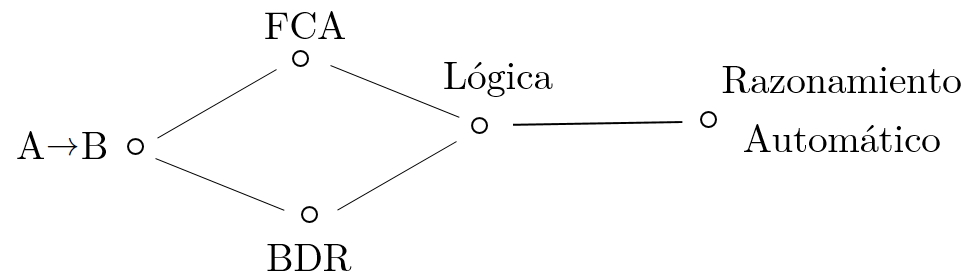
\includegraphics[height=.15\textheight,width=.75\textwidth]{esquemaPreliminares.png}
		\end{center}
		\caption{Esquema de contenido del cap�tulo de Preliminares.}
		\label{figura:esquemaPreliminares}
\end{figure}


\section{An�lisis Formal de Conceptos}
\label{sec:analisisFormalConceptos}
De forma general, se puede considerar FCA como un marco para el an�lisis de informaci�n que facilita la extracci�n de conocimiento y la posibilidad de poder razonar sobre �l. La referencia principal de este campo de conocimiento viene de la mano de Wille y Ganter en \cite{Ganter1997}. Seg�n el propio Wille en \cite{Wille2005}: \textit{``El objetivo y significado del an�lisis formal de conceptos como teor�a matem�tica consiste en apoyar la comunicaci�n racional de las personas, mediante el desarrollo de estructuras de conceptos matem�ticamente apropiadas que puedan activarse l�gicamente''}.

Como principales fortalezas de FCA cabe mencionar: su s�lida base matem�tica y filos�fica, una representaci�n gr�fica e intuitiva del conocimiento, avalada en m�s de 2.000 publicaciones cient�ficas y aplicaciones en cientos de proyectos \cite{Wille2005} en diversos campos de conocimiento, como se ha mencionado en el Cap�tulo \ref{cap:introduccion}. 


\subsection{Contextos formales}
\label{subsec:contextosFormales}
El punto de partida de FCA es un \textit{contexto formal}\index{contexto formal} que se define a continuaci�n.

\begin{definicion}[Contexto formal]
	Un contexto formal es una tripleta $K = (G,M,I)$ que consiste en dos conjuntos no vac�os, $G$ y $M$, y una relaci�n binaria $I$ entre ellos. Los elementos de $G$ se llaman objetos del contexto, y los elementos de $M$ se llaman atributos del contexto. Para $g \in G$ y $m \in M$, escribimos $<g,m> \in I$ o $gIm$ si el objeto $g$ posee el atributo $m$.
\end{definicion}

La forma m�s sencilla de representar un contexto formal es mediante una tabla donde los objetos se sit�an en sus filas y los atributos en las columnas, de forma que un valor en cada celda indica si un objeto $g \in G$ posee un atributo $m \in M$. Hay que tener en cuenta que la definici�n de contexto formal es deliberadamente muy general. No hay restricciones sobre la naturaleza de los objetos y atributos. Se pueden considerar objetos f�sicos, personas, n�meros, procesos, estructuras, etc. En realidad, cualquier cosa que sea un \textit{conjunto} en el sentido matem�tico se puede tomar como el conjunto de objetos o de atributos de alg�n contexto formal. Tambi�n es posible intercambiar el papel de los objetos y atributos, es decir, si se tiene que $K = (G,M,I)$ es un contexto formal, igualmente lo ser� su dual, $K = (M,G,I')$ con $mIg \Longleftrightarrow gIm$. Adem�s, ni siquiera es necesario que $G$ y $M$ sean disjuntos, de hecho, pueden incluso no ser diferentes. Se utilizar�n letras may�sculas: A, B, C, etc., para denotar subconjuntos de $M$ y $G$.

%\begin{ejemplo}
%	Se considera un ejemplo de contexto formal en el cual los objetos son hoteles, los atributos son diferentes servicios que ofrece el establecimiento y cada celda de la tabla indica si un objeto cumple un atributo. Por tanto, se tiene el contexto formal $\mathbf{K} = (G,M,I)$ en el cual:
%
%	G = \{Fuerte Estepona Suites, Hotel Buenavista, Hotel Para�so, Apts Marriot Playa, Hotel Piedra Paloma, Hostal Hospeder�a V Cent\}
%
%	M = \{AC, Bar, Gimnasio, Internet, Masajes, Aparcamiento\}
%
%	La Tabla \ref{table:hotelsExtract} muestra la relaci�n binaria $I$ utilizando informaci�n real de varios hoteles de la Costa del Sol.
%
%\begin{table*}[tb]
%\caption{Ejemplo de contexto formal utilizando datos reales del sector hotelero}
%\label{table:hotelsExtract} 
%\centering
%{\scriptsize
%\begin{tabular}{lccccccccc}
%\hline
% & AC & Bar & Gimnasio & Internet & Masajes & Aparcamiento\\
%\hline
%Fuerte Estepona Suites & \checkmark & \checkmark & \checkmark & \checkmark & \checkmark & \checkmark\\
%Hotel Buenavista &  & \checkmark &  &  &  & \checkmark \\
%Hotel Para�so & \checkmark & \checkmark &  &  &  & \checkmark \\
%Apts Marriot Playa &  &  &  & \checkmark &  &  \\
%Hotel Piedra Paloma &  & \checkmark &  &  &  & \checkmark \\
%Hostal Hospeder�a V Cent & \checkmark & \checkmark &  & \checkmark &  & \checkmark \\
%\hline
%\end{tabular}
%}
%\end{table*}
%
%	%Por tanto, se puede apreciar como el hotel \textit{Fuerte Estepona Suites} ofrece todos los servicios disponibles en el contexto, mientras que los \textit{Apts Marriot Playa} �nicamente ofrecen el servicio de \textit{Internet}.
%\end{ejemplo}

Para ilustrar un ejemplo de contexto formal\index{contexto formal} y como apoyo al contenido que se presenta en esta secci�n, se va a utilizar el siguiente ejemplo tomado de \cite{Ganter2002}. En �l, los autores muestran un informaci�n sobre los destinos a�reos que oferta un grupo de aerol�neas comerciales.

\begin{ejemplo}
\label{ejemploContextoFormal}
	Sea $K$ un contexto formal donde el conjunto de objetos $G$ comprende todas las l�neas a�reas del grupo Star Alliance y el conjunto de atributos $M$ muestra sus destinos.
	
	La relaci�n binaria $I$ viene reflejada en la Tabla \ref{tabla:ejemploContextoFormal} y muestra los destinos a los que viaja cada miembro de Star Alliance. Por tanto, se tiene el contexto formal $K = (G,M,I)$ en el cual:

	G = \{Air Canada, Air New Zealand, All Nippon Airways, Ansett Australia, The Austrian Airlines Group, British Midland, Lufthansa, Mexicana, Scandinavian Airlines, Singapore Airlines, Thai Airways International, Unites Airlines, VARIG\}

	M = \{Latinoam�rica, Europa, Canad�, Asia, Oriente Medio, �frica, M�xico, Caribe, Estados Unidos\}

\begin{table*}[tb]
\caption{Ejemplo de contexto formal sobre los destinos a�reos del grupo Star Alliance \cite{Ganter2002}}
\label{tabla:ejemploContextoFormal} 
\centering
{\scriptsize
\begin{tabular}{lccccccccc}
\hline
 & \rotatebox{90}{Latinoam�rica} & \rotatebox{90}{Europa} & \rotatebox{90}{Canad�} & \rotatebox{90}{Asia} & \rotatebox{90}{Oriente Medio} & \rotatebox{90}{�frica} & \rotatebox{90}{M�xico} & \rotatebox{90}{Caribe} & \rotatebox{90}{Estados Unidos\ }\\
\hline
Air Canada & \checkmark & \checkmark & \checkmark & \checkmark & \checkmark &  & \checkmark & \checkmark & \checkmark\\
Air New Zealand &  & \checkmark &   & \checkmark  & & & & & \checkmark \\
All Nippon Airways &  & \checkmark &   & \checkmark  & & & & & \checkmark \\
Ansett Australia  &  &  &   & \checkmark  & & & & & \\
The Austrian Airlines Group &  & \checkmark & \checkmark & \checkmark & \checkmark & \checkmark &  &  & \checkmark\\
British Midland &  & \checkmark &  &  &  &  &  &  & \\
Lufthansa & \checkmark & \checkmark & \checkmark & \checkmark & \checkmark & \checkmark & \checkmark &  & \checkmark\\
Mexicana & \checkmark &  & \checkmark &  &  &  & \checkmark & \checkmark & \checkmark\\
Scandinavian Airlines & \checkmark & \checkmark &  & \checkmark &  & \checkmark &  &  & \checkmark\\
Singapore Airlines &  & \checkmark & \checkmark & \checkmark & \checkmark & \checkmark &  &  & \checkmark\\
Thai Airways International & \checkmark & \checkmark &  & \checkmark &  &  &  & \checkmark & \checkmark\\
Unites Airlines & \checkmark & \checkmark & \checkmark & \checkmark &  &  & \checkmark & \checkmark & \checkmark\\
VARIG & \checkmark & \checkmark &  & \checkmark &  & \checkmark & \checkmark &  & \checkmark\\
\hline
\end{tabular}
}
\end{table*}
\end{ejemplo}


\subsection{Operadores de derivaci�n}
\label{subsec:operadoresDerivacion}
Dada una selecci�n $A \subseteq G$ de objetos de un contexto formal\index{contexto formal} $K = (G,M,I)$, se desea caracterizar qu� atributos de $M$ son comunes a todos estos objetos. Esto define un operador que produce para cada conjunto de objetos $A \subseteq G$, el conjunto $A$ de sus atributos comunes, y dualmente, a partir de un conjunto de atributos, caracterizar el conjunto de atributos que tienen en com�n a dichos atributos. Estos operadores se denominan operadores de derivaci�n\index{operadores de derivaci�n} para $K$.
 
\begin{definicion}[Operadores de derivaci�n]
	Dado un contexto formal $K = (G,M,I)$, se definen los operadores de derivaci�n:

$$
\begin{array}{ll}
(\ )'\colon 2^G  \to 2^M
&
(\ )'\colon 2^M  \to 2^G
\\[2mm]
A' = \{m \in M \mid g\I m  \quad \forall g \in A\}\qquad
&
B' = \{g \in G \mid g\I m  \quad \forall m \in B\}
\end{array}
$$
\end{definicion}

Ambas funciones se denotan con el mismo s�mbolo porque no hay lugar a confusi�n.

Si $A$ es un conjunto de objetos, entonces $A'$ es un conjunto de atributos, al cual podemos aplicar el segundo operador de derivaci�n para obtener el conjunto de objetos $A''$. De forma dual, comenzando con un conjunto $B$ de atributos, podemos formar el conjunto de atributos $B''$.

De la definici�n anterior se obtiene que:

%\begin{proposicion}
%	Sean los subconjuntos $A, A_1, A_2 \subseteq G$, se tiene que:
%	\begin{enumerate}
%		\item $A_1 \subseteq A_2 \Rightarrow A^{'}_2 \subseteq A^{'}_1$
%		\item $A \subseteq A''$
%		\item $A = A''''$
%	\end{enumerate}
%\end{proposicion}

El operador de cierre $''$ (i.e. aplicar el operador de derivaci�n $'$ y su dual) verifica algunas propiedades interesantes que ser�n fundamentales para poder desarrollar la teor�a formal.

\begin{definicion}[Operador de cierre]\index{operador de cierre}
	Sea $K\ =\ (G,M,I)$ un contexto formal, entonces el operador $()'' : 2^G \to 2^G$ es un operador de cierre, es decir, satisface las siguientes propiedades:
	\begin{itemize}
		\item Idempotente: $X'''' = X'' \quad \forall X \in 2^M$
		\item Mon�tona: $X \subseteq Y$ $\rightarrow$ $X'' \subseteq Y'' \quad \forall X,Y \in 2^M$ 
		\item Extensiva: $X \subseteq X'' \quad \forall X \in 2^M$
	\end{itemize}
	
Por dualidad, el resultado es igualmente v�lido para $()'' : 2^M \to 2^M$.
\end{definicion}

Un conjunto $A \subseteq M$ se denomina \textit{conjunto cerrado} para el operador $''$ si es un punto fijo para $''$, es decir, $A''=A$. Los conjuntos cerrados\index{conjuntos cerrados} permiten definir lo que se denominan \textit{conceptos formales}\index{concepto formal}, los cuales son una noci�n esencial en FCA y a los que se dedica el siguiente apartado. 


\subsection{Conceptos Formales}
\label{subsec:conceptosFormales}
De forma general, un concepto formal permite describir formalmente un hecho del contexto y caracterizar un conjunto de objetos por medio de los atributos que comparten y viceversa. 

As�, un par $(X,Y)$ con $X\subseteq G$ y $Y\subseteq M$ es un concepto formal cuando se verifica que:
\begin{itemize}
	\item Cada objeto en $X$ tiene todos los atributos de $Y$, y dualmente, cada atributo de $Y$ est� presente en cada objeto de $X$.
	\item Para cada objeto en $G$ que no est� en $X$, existe un atributo en $Y$ que el objeto no tiene. Dualmente, para cada atributo en $M$ que no est� en $Y$, hay un objeto en $X$ que no tiene ese atributo.
\end{itemize}

Se introduce ahora la noci�n formalmente:

\begin{definicion}[Concepto formal]
	Sea $K = (G,M,I)$ un contexto formal\index{contexto formal} y $A \subseteq G$, $B \subseteq M$. El par (A, B) se denomina concepto formal si $A'=B$ y $B'=A$. El conjunto de objetos $A$ se denomina extensi�n del concepto (A, B) mientras que el conjunto de atributos $B$ ser� la intensi�n del concepto.
\end{definicion}

La descripci�n de un concepto a trav�s de su extensi�n e intenci�n es redundante, ya que cada una de las dos partes determina la otra debido a que $B\ =\ A'$ y $A\ =\ B'$, sin embargo, pueden existir ocasiones en las cuales esta descripci�n redundante puede ser conveniente \cite{Ganter2002}.

Una alternativa gr�fica de identificar los conceptos formales es la siguiente. Desde la representaci�n del contexto formal, un concepto formal se puede reconocer por medio de una submatriz de tal manera que se verifican todas las relaciones contenidas en la submatriz (no es necesario que la submatriz est� formada por celdas contiguas). De esta forma, en la Tabla \ref{tabla:extractoEjemploContextoFormal}, se ve como es posible identificar el concepto formal construido con el par (\textit{\{Air New Zealand, All Nippon Airways\},\{Europa, Asia, Estados Unidos\}}) a partir del contexto formal. 

%\begin{table*}[tb]
%\caption{Conceptos formales a partir de la representaci�n del contexto formal.}
%\label{table:conceptosFormales} 
%\centering
%{\scriptsize
%\begin{tabular}{lcccccc}
%\hline
%Modelo de coche & Consumo & Cilindrada & Movilidad & Potencia & Peso & Aceleraci�n\\
%\hline
%Chevrolet Vega &  &  &  & \checkmark &  & \checkmark\\
%Toyota Corolla &  &  &  & \checkmark &  & \\
%Ford Pinto &  &  & \checkmark &  & \checkmark & \\
%Volkswagen Beetle & \checkmark &  & \checkmark & \checkmark & \checkmark & \checkmark \\
%Plymouth Satellite  & \cellcolor{gray!25}\checkmark & \cellcolor{gray!25}\checkmark & \cellcolor{gray!25}\checkmark &  &  & \cellcolor{gray!25}\checkmark \\
%Chevrolet Malibu & \cellcolor{gray!25}\checkmark & \cellcolor{gray!25}\checkmark & \cellcolor{gray!25}\checkmark &  &  & \cellcolor{gray!25}\checkmark \\
%\hline
%\end{tabular}
%}
%\end{table*}

\begin{table*}[tb]
\caption{Extracto del ejemplo de contexto formal sobre los destinos a�reos del grupo Star Alliance \ref{tabla:ejemploContextoFormal}}
\label{tabla:extractoEjemploContextoFormal} 
\centering
{\scriptsize
\begin{tabular}{lccccccccc}
\hline
 & \rotatebox{90}{Latinoam�rica} & \rotatebox{90}{Europa} & \rotatebox{90}{Canad�} & \rotatebox{90}{Asia} & \rotatebox{90}{Oriente Medio} & \rotatebox{90}{�frica} & \rotatebox{90}{M�xico} & \rotatebox{90}{Caribe} & \rotatebox{90}{Estados Unidos\ }\\
\hline
$\left [ \ldots \right ]$ &  &  &  &  &  &  &  &  & \\
\cellcolor{gray!25}Air New Zealand &  & \cellcolor{gray!25}\checkmark &   & \cellcolor{gray!25}\checkmark  & & & & & \cellcolor{gray!25}\checkmark \\
\cellcolor{gray!25}All Nippon Airways &  & \cellcolor{gray!25}\checkmark &   & \cellcolor{gray!25}\checkmark  & & & & & \cellcolor{gray!25}\checkmark \\
$\left [ \ldots \right ]$  &  &  &  &  &  &  &  &  & \\
\hline
\end{tabular}
}
\end{table*}


\subsection{Ret�culo de conceptos}
\label{subsec:reticuloConceptos}
Un contexto formal\index{contexto formal} puede tener muchos conceptos formales. El conjunto de todos los conceptos formales de un contexto formal $K$ tiene estructura de \textit{ret�culo} con la relaci�n de orden que se muestra a continuaci�n.

Si $(X_1,Y_1)$ y $(X_2,Y_2)$ son conceptos, se define un orden parcial, $\leq$, de forma que $(X_1,Y_1) \leq (X_2,Y_2)$ si y s�lo si $X_1 \subseteq X_2$, o equivalentemente, si $Y_2 \subseteq Y_1$.

%Los pares de conceptos en este orden parcial tienen una �nica m�xima cota inferior, que es el concepto generado por $X_1 \cap X_2$. De forma an�loga, poseen una �nica m�nima cota superior, el concepto generado por los atributos $Y_1 \cap Y_2$. Por medio de estas operaciones de c�lculo del m�ximo y del m�nimo de dos conceptos, se satisfacen las propiedades que definen un ret�culo. 

La Figura \ref{figura:ejemploReticuloAerolineas} muestra el ret�culo de conceptos\index{ret�culo de concepto} asociado al contexto formal mostrado anteriormente \ref{ejemploContextoFormal}.

\begin{figure}[htbp]
		\begin{center}
			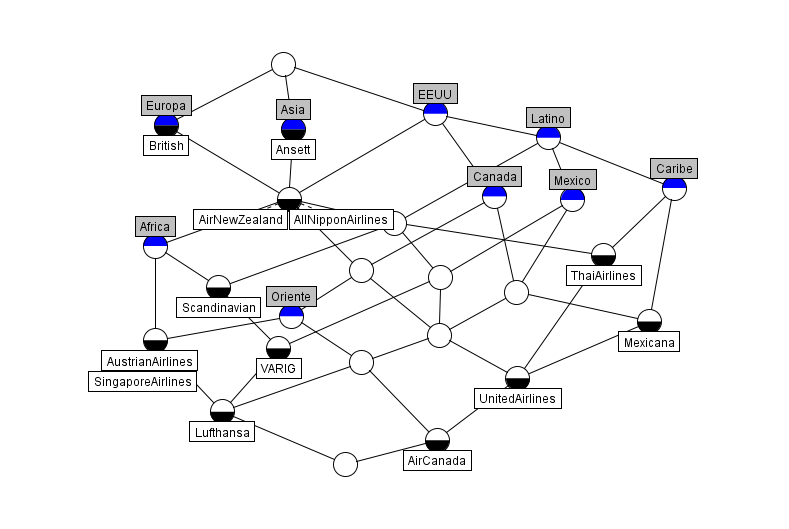
\includegraphics[height=.6\textheight,width=1\textwidth]{ejemploReticuloAerolineas.png}
		\end{center}
		\caption{Ret�culo de conceptos\index{ret�culo de conceptos} asociado al contexto formal \ref{ejemploContextoFormal}}
		\label{figura:ejemploReticuloAerolineas}
\end{figure}

En un diagrama como el de la Figura \ref{figura:ejemploReticuloAerolineas}, cada nodo representa un concepto formal. Un concepto $c_1$ es un subconcepto de un concepto $c_2$ si y solo si hay un camino de  descendente desde el nodo que representa $c_2$ al nodo que representa $c_1$. El nombre de un objeto $g$ se asocia al nodo que representa el concepto m�s peque�o que contiene $g$ en su extensi�n; dualmente, el nombre de un atributo $m$ va asociado al nodo que representa el concepto m�s grande con $m$ en su intensi�n. 

Se pueden comprobar f�cilmente las relaciones que existen en el contexto ya que un objeto $g$ tiene un atributo $m$ si y solo si el concepto asociado a $g$ es un \textit{subconcepto} del asociado a $m$. La extensi�n de un concepto consiste en todos aquellos objetos cuyas etiquetas est�n asociadas a subconceptos, y, dualmente, la intensi�n consiste en todos los atributos asociados a \textit{superconceptos}. 

Dicho lo anterior y teniendo en cuenta la sobrecarga que conllevar�a representar cada concepto del ret�culo en la Figura \ref{figura:ejemploReticuloAerolineas}, se puede mencionar aqu� como ejemplo, el concepto etiquetado como `Oriente Medio' \textit{(Middle East)}, el cual tiene como extensi�n el conjunto \{\textit{Singapore Airlines, The Austrian Airlines Group, Lufthansa, Air Canada}\}, y como intensi�n \{\textit{Middle East, Canad�, Estados Unidos, Europa, Asia}\}.

En la parte superior del ret�culo, encontramos los destinos que ofrecen la mayor�a de las aerol�neas: Europa, Asia Pac�fico y los Estados Unidos. Por ejemplo, exceptuando British Midland y Ansett Australia, todas las aerol�neas ofrecen vuelos a Estados Unidos. Esas dos l�neas a�reas se encuentran en la parte superior del diagrama, ya que tienen la menor oferta de vuelos, operan s�lo en Europa y Asia, respectivamente. 

De esta forma, cuanto m�s se descienda en el ret�culo de conceptos, m�s destinos ofrecer�n las aerol�neas. As�, la mayor oferta de destinos se encuentra en las aerol�neas de la parte inferior del ret�culo: Lufthansa y Air Canada. De forma an�loga, cuanto m�s se descienda en el ret�culo, ser�n menos los destinos ofertados, e.g. �frica, Oriente Medio y el Caribe.



\subsection{Sistema de implicaciones}
\label{subsec:sistemaImplicaciones}
Una noci�n equivalente al ret�culo de conceptos es el denominado sistema de implicaciones \cite{Ganter1997}. Como ya se adelant� en el Cap�tulo \ref{cap:introduccion}, las implicaciones constituyen el eje fundamental de trabajo en esta tesis doctoral. Reflejan una forma relativamente sencilla de representar las relaciones l�gicas que se encuentran entre los atributos que poseen los objetos del contexto formal ya que combinan una forma muy simple y natural de escribir reglas del tipo \textit{si-entonces}\index{if-then rules} con una gesti�n automatizada de la informaci�n.

Para introducir el trabajo realizado utilizando la l�gica sobre los conjuntos de implicaciones, se va a proceder describiendo los componentes habituales de una l�gica: su lenguaje, sem�ntica, sistema axiom�tico y m�todo de razonamiento autom�tico. No obstante, como se ha comentado anteriormente, los conjuntos de implicaciones se han utilizado para diferentes campos de conocimiento (FCA, bases de datos y sistemas de recomendaci�n). En consecuencia, en este punto se presentan los elementos de la l�gica que ser�n comunes a todos ellos, en concreto, el lenguaje. El resto se presentar� para cada una de las secciones correspondientes \ref{sec:basesDatosRelacionales} y \ref{sec:logicaSimplificacion}.

\subsection*{Lenguaje}
\noindent
\begin{definicion}
	Dado un conjunto $M$ finito de s�mbolos (denominados atributos) no vac�o, el lenguaje sobre $M$ se define como: 
$$
\mathcal L_M = \{A\to B\mid A,B\subseteq M\}
$$
\end{definicion}

Las f�rmulas $A \to B$ se denominan \emph{implicaciones} y los conjuntos $A$ y $B$ reciben el nombre de \emph{premisa} y \emph{conclusi�n} de la implicaci�n\index{Implicaci�n} respectivamente. Los conjuntos $\sum \subseteq \mathcal L_M$ se denominan \emph{sistemas de implicaciones} sobre $M$.

Se utilizar� la siguiente notaci�n:
\begin{itemize}
	\item Se utilizar�n letras min�sculas para denotar los elementos en $M$, mientras que las may�sculas denotan sus subconjuntos.
	\item Se omiten las llaves en premisas y conclusiones, es decir, $abcde$ denota el conjunto $\{a,b,c,d,e\}$.
	\item Se escriben los elementos de $2^M$ por yuxtaposici�n, es decir, para $X \cup Y$ se escribir� $XY$.
	\item Para la diferencia, se utiliza $X-Y$ por $X \smallsetminus Y$.
\end{itemize}

%\begin{definicion}[Implicaci�n]\index{Implicaci�n}
%	Una implicaci�n sobre un conjunto de atributos $M$ es una expresi�n de la forma $X \to Y$, donde $X$ e $Y$ son conjuntos de atributos, i.e. $X \subseteq M$ y $Y \subseteq M$.
%\end{definicion}

\begin{definicion}[Implicaci�n trivial]\index{Implicaci�n!trivial}
	Una implicaci�n $X \to Y$ es trivial si $Y \subseteq X$.
\end{definicion}

\begin{definicion}[Implicaci�n unitaria]\index{Implicaci�n!unitaria}
	Una implicaci�n se dice unitaria si su conclusi�n es un conjunto unitario, i.e. $X \to a$.
\end{definicion}


\subsection*{Sem�ntica}
\noindent
Tras la definici�n del lenguaje se pasa ahora a introducir la sem�ntica utilizada, para lo cual se va a utilizar el concepto de \textit{operador de cierre}\index{operador de cierre} definido anteriormente.

%Un operador de cierre $c$ en $M$ recibe el nombre de \emph{modelo} para una implicaci�n $A\to B\in\mathcal L_M$ si $B\subseteq  c(A)$; se denota $c\models A\to B$. Adem�s, dado un sistema de implicaciones $\Sigma\subseteq \mathcal L_M$ y un operador de cierre $c$ en $M$, $c\models \Sigma$ denota que $c\models A\to B$ para todo $A\to B\in \Sigma$.

%Se dice que una implicaci�n $X \to Y$ se cumple en un contexto formal $K$ si y s�lo si cada objeto $A \in G$ que tiene todos los atributos de $X$ tambi�n tiene todos los atributos de $Y$.

%En definitiva, $\Sigma \models A\to B$ si cada modelo de $\Sigma$ es un modelo para $A\to B$, y $\Sigma_1 \equiv \Sigma_2$ si sus modelos representan el mismo conocimiento.

\begin{definicion}[Modelo]\index{Modelo}
	Sea $K=(G,M,I)$ un contexto formal\index{contexto formal} y sea $A\to B \in \mathcal L_M$. El contexto K es un modelo para $A\to B$ si $B \subseteq A''$. Se denota por $K\models A\to B$.
\end{definicion}

La noci�n de modelo puede extenderse a los sistemas de implicaciones de la siguiente manera. Dado $\Sigma\subseteq \mathcal L_M$, la expresi�n $K\models \Sigma$ indica que $\Sigma \models A\to B$ para toda $A \to B \in \Sigma$.

\begin{ejemplo}
	De la informaci�n mostrada en el contexto formal \ref{tabla:ejemploContextoFormal} se puede identificar que: $K \models Caribe \to Latinoamerica$. Y tambi�n que: $K \not\models Caribe \to Mexico$.
\end{ejemplo} 

\begin{ejemplo}
	Sea $M = \{a,b,c,d\}$ un conjunto de atributos. Se cumple que $\{a\to b, a\to c\} \equiv \{a\to bc\}$ porque para cada contexto formal $K = (G,M,I)$, se verifica que $\{b,c\}' = \{b\}' \cup \{c\}'$. Por tanto, $\{a\}' \subseteq \{b\}'$ y $\{a\}' \subseteq \{c\}'$ si y s�lo si $\{a\}' \subseteq \{b,c\}'$.
\end{ejemplo}

\begin{proposicion}
	Sea $M$ un conjunto de atributos y $\Sigma \subseteq \mathcal L_M$. Se verifica que:
	\[
		\Sigma \equiv \bigcup_{A\to B \in \Sigma} \{A \to b \mid b \in B\}
	\]
\end{proposicion}

Un ejemplo b�sico de implicaciones puede verse utilizando nuevamente la informaci�n de la Tabla \ref{tabla:ejemploContextoFormal}. En ese ejemplo puede apreciarse una relaci�n que siempre se cumple y es la siguiente. Si la aerol�nea provee servicio de vuelo a \textit{Latinoam�rica} entonces tambi�n ofrece como destino \textit{Estados Unidos}. He ah� un claro ejemplo de regla \textit{si-entonces} o implicaci�n (en este caso, unitaria), que se verifica en el contexto.

Las implicaciones se interpretan de forma conjuntiva, es decir, corresponden a las f�rmulas $a_1\land \ldots\land a_n \to b_1\land \ldots\land b_m$ donde las proposiciones $a_1, \ldots  a_n,  b_1, \ldots, b_m$ son elementos del conjunto $M$.

%Por completitud, el conjunto de todas las implicaciones que se verifican en ese contexto es: 
%
%\noindent
%$\Sigma\ =\ \{$ 
%
%$Europa,\ Estados\  Unidos \rightarrow Asia$;
%
% $Asia,\  Estados\  Unidos \rightarrow Europa$; 
% 
% $Latinoamerica \rightarrow Estados\  Unidos$; 
% 
% $Canada \rightarrow Estados\  Unidos$; 
% 
% $Europa,\  Asia \rightarrow Estados\  Unidos$;  
% 
% $Africa \rightarrow Europa,\  Asia,\  Estados\  Unidos$; 
% 
% $Mexico \rightarrow Latinoamerica,\  Estados\  Unidos$; 
% 
% $Caribe \rightarrow Latinoamerica,\  Estados\  Unidos$; 
% 
% $Latinoamerica,\  Canada,\  Estados\  Unidos \rightarrow Mexico$; 
% 
% $Europa,\  Canada,\  Asia,\  Africa,\  Estados\  Unidos \rightarrow Oriente\  Medio$; 
% 
% $Oriente\  Medio \rightarrow Europa,\  Canada,\  Asia,\  Estados\  Unidos$;
% 
% $Latinoamerica,\  Mexico,\  Caribe,\  Estados\  Unidos \rightarrow Canada$
% 
%\noindent
% $\}$.

Al comenzar el cap�tulo se habl� de la equivalencia entre el ret�culo de conceptos y las implicaciones; tras haber introducido formalmente el lenguaje y la sem�ntica de las implicaciones, ahora ya se pueden mencionar ejemplos de esta equivalencia utilizando la informaci�n del ret�culo \ref{figura:ejemploReticuloAerolineas}. As�, es posible identificar ejemplos de implicaciones tales como:

$\{Canada \rightarrow Estados\  Unidos,$

$Oriente\  Medio \rightarrow Europa,\  Canada,\  Asia,\  Estados\  Unidos\}$;

Se puede considerar a las implicaciones y el ret�culo de conceptos como distintas alternativas de tratar la informaci�n que se puede extraer de un contexto formal\index{contexto formal}. No obstante, los ret�culos de conceptos permiten una representaci�n gr�fica, mientras que la caracter�stica fundamental, desde el punto de vista de esta tesis doctoral, es que los sistemas de implicaciones proporcionan una manipulaci�n simb�lica usando la l�gica de implicaciones, y por tanto, permiten el razonamiento autom�tico.

Como se ha mencionado anteriormente, se entra ahora en la segunda secci�n de este cap�tulo en la cual se van a utilizar las implicaciones en el entorno de las bases de datos relacionales, donde recibir�n el nombre de Dependencias Funcionales.



\section{Bases de Datos Relacionales}\index{Bases de Datos Relacionales}
\label{sec:basesDatosRelacionales}
El modelo de base de datos relacional aparece en el exitoso art�culo de Edgar Frank Codd en 1970 \cite{Codd1970}. Codd propuso que los sistemas de bases de datos deber�an presentarse al usuario con una vista de datos organizada en forma de tablas bidimensionales (filas y columnas) que denomin� \textit{relaciones}. La Tabla \ref{tabla:ejemploPeliculas} es un ejemplo de relaci�n en el que cada fila representa una pel�cula y cada columna una propiedad de la pel�cula. 

En un esquema relacional se pueden encontrar los siguientes elementos:
\begin{itemize}
	\item \textbf{Atributo}\index{atributo}. Cada una de las columnas de un relaci�n se denomina atributo. En el ejemplo \ref{tabla:ejemploPeliculas} los atributos son: T�tulo, A�o, Pa�s, Director, Nacionalidad, Actor.
	\item \textbf{Tupla}\index{tupla}. Se denomina tupla a cada fila de una relaci�n exceptuando la fila que contiene a los atributos.
	\item \textbf{Dominio}\index{dominio}. El modelo relacional requiere que cada componente de cada tupla sea at�mico. No se permite que un valor de la tupla sea una estructura de datos (e.g. una lista, una matriz, un conjunto, etc.) cuyos valores puedan dividirse en componentes m�s peque�os. De esta forma, se establece que cada atributo de la relaci�n est� asociado a un dominio, i.e. un tipo particular de dato.
\end{itemize}

%Las relaciones son conjuntos de tuplas, no listas de tuplas y por tanto, el orden en que el se presenten las tuplas de una relaci�n es irrelevante. De hecho, se puede incluso modificar el orden de aparici�n de los atributos y la relaci�n se mantiene constante.

Formalmente, en el modelo relacional, una base de datos consiste en una o m�s relaciones \cite{Elmasri2010}. La planificaci�n de la estructura de la base de datos, en particular de las relaciones, es vital para la gesti�n efectiva de la misma \cite{Harrington2016}. Una relaci�n $R$ definida sobre un conjunto de dominios $D_1$, $D_2$, ..., $D_n$ est� formada por un esquema y un cuerpo como se definen a continuaci�n.

\begin{definicion}[Esquema]\index{Esquema}
	Un esquema $E$ para una relaci�n $R$ se define como un conjunto fijo de pares \textit{(atributo:dominio)}. Habitualmente se denota como $\{(A_1:D_1),\ (A_2:D_2),\ (A_n:D_n)\}$ donde cada $A_j$ corresponde a un �nico $D_j$ y los $A_j$ son todos distintos.
\end{definicion}

En el ejemplo \ref{tabla:ejemploPeliculas}, el esquema ser�a: 

\noindent
\textit{\{}

\textit{T�tulo:Cadena de caracteres, A�o:N�mero natural, Pa�s:Cadena de caracteres, Director:Cadena de caracteres, Nacionalidad:Cadena de caracteres, Actor:Cadena de caracteres}

\noindent
\textit{\}}.

El conjunto de los esquemas para las relaciones de una base de datos se denomina \textit{esquema de base de datos relacional}.

\begin{definicion}[Cuerpo]\index{Cuerpo}
	Un cuerpo $C$ para una relaci�n $R$ se define como un conjunto de tuplas de pares \textit{(atributo:valor)}. Habitualmente se denota como $\{(A_1:v_{i1}),\ (A_2:v_{i2}),\ (A_n:v_{in})\}$ con $i = 1,2,...,m$ tal que $m$ es el cardinal de $R$, i.e. el n�mero de tuplas de la relaci�n. En cada $(A_j:v_{ij})$ se tiene que $v_{ij} \in D_j$.
\end{definicion}

En el ejemplo \ref{tabla:ejemploPeliculas}, un extracto del cuerpo ser�a:

\noindent
\textit{\{}

	\textit{[(T�tulo:Pulp Fiction), (A�o:1994), (Pa�s:USA), (Director:Quentin Tarantino), (Nacionalidad:USA), (Actor:Uma Thurman)],}

 \textit{[(T�tulo:King Kong), (A�o:2005), (Pa�s:NZ), (Director:Peter Jackson), (Nacionalidad:NZ), (Actor:Naomi Watts)], }
 
 \textit{...}
 
\noindent
\textit{\}}.

%Un dise�o impreciso de un esquema de base de datos relacional puede generar ciertas anomal�as que provoquen el mal funcionamiento del sistema. Una anomal�a es una inconsistencia entre una parte de los datos y otra. Los principales tipos de anomal�as aparecen a la hora de operar con el sistema en t�rminos de actualizaciones, eliminaciones o inserci�n de informaci�n redundante \cite{Vavilis2015,Costante2017}.



\subsection{Dependencias Funcionales}
\label{subsec:dependenciasFuncionales}
Existen muchas restricciones que el modelo relacional permite establecer en las relaciones de los esquemas de la base de datos. Concretamente, esta parte de la tesis est� enfocada en las restricciones denominadas dependencias funcionales.

\begin{definicion}[Dependencia Funcional]\index{dependencias funcionales}
	Sea M un conjunto de atributos. Una dependencia funcional (FD) sobre M es una expresi�n de la forma $X \rightarrow Y$, donde $X,\ Y$ son conjuntos de atributos.
\end{definicion}

Teniendo en cuenta que la sintaxis que se va a utilizar para FD es la misma que para implicaciones, existen tipos de FD denominados triviales y unitarias, cuyas nociones son iguales a las introducidas para implicaciones en \ref{subsec:sistemaImplicaciones}. Se pasa ahora a describir la sem�ntica para las FD.

%\begin{definicion}[Dependencia Funcional Trivial]
%	Una dependencia funcional es trivial si $X \subseteq Y$.
%\end{definicion}
%
%\begin{definicion}[Dependencia Funcional Unitaria]
%	Una dependencia funcional es unitaria cuando su conclusi�n es un conjunto unitario, es decir, $X \rightarrow a \ \mid \ a \in M$.
%\end{definicion}
%
%\begin{definicion}[Esquema Relacional]
%	Un esquema de relaci�n \df es un par ordenado que consiste en un conjunto de atributos $M$ y un conjunto $F$ de FD sobre $M$.
%\end{definicion}

\subsection*{Sem�ntica}
\noindent
Una FD se satisface en una tabla $R$ si para cada dos tuplas\index{tupla} de $R$, si verifican $X$, entonces verifican $Y$. Intuitivamente, una FD $X \rightarrow Y$ indica que el conjunto de atributos $X$ determina el conjunto de atributos $Y$, lo cual refleja fielmente el concepto de regla \textit{si-entonces} que definen las implicaciones y se acerca a la definici�n de una funci�n entre los dominios de $A$ y $B$, $f: A\to B$. Entonces, �por qu� el cambio de denominaci�n? 

En la Secci�n \ref{subsec:sistemaImplicaciones} se defini� la noci�n de implicaci�n, denotado por $X \rightarrow Y$, y se dijo que una implicaci�n se verifica en un contexto formal\index{contexto formal} $K$ si cada objeto del contexto que contenga los atributos de $X$ tambi�n tiene los de $Y$, sin embargo, en una FD, no s�lo esos atributos tienen que aparecer en ambos conjuntos sino que adem�s su \textit{valor} ha de ser el mismo.

Esta es una diferencia esencial que surge del hecho de que en contextos formales se trata con una relaci�n binaria $I$ entre los objetos y los atributos del contexto, mientras que en esquemas relacionales, los atributos pueden ser valores \textit{multivaluados} y por tanto, para que una FD se verifique, han de coincidir los valores  de la relaci�n.

Para ilustrar de una forma m�s sencilla esta diferencia vamos a utilizar el siguiente ejemplo:
\begin{ejemplo}
Sea el contexto formal $K=(G,M,I)$ representado en \ref{tabla:ejemploContextoFormal} donde los objetos son $g_i \in G$ y los atributos $a,b,c \in G$.

Seg�n la definici�n de implicaci�n \ref{subsec:sistemaImplicaciones}, se puede ver como se verifica la implicaci�n $a \to c$ en $K$, mientras que por el contrario, al considerar la relaci�n como una tabla del modelo relacional y considerando la definici�n de FD, no se cumple que $a \to c$ debido al �ltimo objeto $g_4$. 
	\begin{table*}[htbp]
	\caption{Ejemplo de contexto formal para ilustrar la diferencia entre implicaci�n y dependencia funcional}
	\label{tabla:ejemploContextoFormal}
	\centering
	{\scriptsize
	\begin{tabular}{cccccc}
 		%\hline
  	& a & b & c \\
 		\hline
 		$g_1$ & 1 & 0 & 1\\
 		$g_2$ & 1 & 1 & 1\\
 		$g_3$ & 0 & 0 & 0\\
 		$g_4$ & 0 & 1 & 1\\
 		%\hline
	\end{tabular}
	}
\end{table*}
\end{ejemplo}

%Para ilustrar de una forma m�s sencilla esta diferencia se puede contrastar la informaci�n que refleja el contexto formal del ejemplo \ref{tabla:ejemploContextoFormal} con la Tabla \ref{tabla:ejemploPeliculas}. En el primero se ve como los valores de la relaci�n pueden considerarse binarios en el sentido de que indican si una aerol�nea ofrece vuelo a un destino o no. Sin embargo, en el segundo, la tabla refleja diferentes valores para cada uno de los atributos del esquema (nombres propios, a�os, etc.). 

%De esta manera, una implicaci�n que verifica en ese contexto formal es $Canada \rightarrow Estados\ Unidos$, mientras que una FD que se verifica en el esquema relacional puede ser $Director \rightarrow Nacionalidad$. Sin embargo, n�tese que por contra, la FD $Director \rightarrow Titulo$ no es v�lida pues existe m�s de una tupla de la relaci�n cuyos valores para esos atributos no coinciden, Quentin Tarantino dirige tanto \textit{Pulp Fiction} como \textit{Django Unchained}.

El concepto de implicaciones en FCA puede ampliarse para poder tratar con contextos formales donde la relaci�n $I$ toma valores en un conjunto en lugar de ser binaria. Este tipo de contextos formales\index{contexto formal} se denominan multivaluados y su aproximaci�n se realiza a trav�s del llamado an�lisis de conceptos formales difusos \cite{Burusco1998,Belohlavek2000}, lo que queda fuera del �mbito de esta tesis doctoral.

%tratar situaciones multivaluadas otorgando valores, por ejemplo, dentro de un rango [0,1], pero en ese caso, se entrar�a en lo que se denomina implicaciones difusas  \cite{Baczynski2008} que es otro campo de conocimiento que queda fuera del �mbito de esta tesis doctoral.

Como consecuencia de lo anterior, la noci�n de FD es de gran importancia en la tesis debido a que es la base para el trabajo realizado sobre el problema de la enumeraci�n de todas las claves minimales de esquemas relacionales.

Una clave en bases de datos relacionales est� constituida por un subconjunto de los atributos del esquema de una tabla tal que los valores de esos atributos identifican un�vocamente a cada tupla de la tabla. Se puede definir por medio de FD de la siguiente forma:

\begin{definicion}[Clave]\index{clave}
	Dada una tabla $R$ sobre el conjunto de atributos $M$, se dice que $K \subseteq M$ es una clave de $R$ si la FD $K \rightarrow M$ se verifica en $R$.
\end{definicion}

\begin{definicion}[Clave Minimal]\index{clave!claves minimales}
	Dada una tabla $R$, el conjunto de atributos $K \subseteq M$ se dice que es una clave minimal si $K$ es clave y para todo atributo $k \in K$ el subconjunto $K - \{k\}$ no es clave de $R$.
\end{definicion}

\begin{definicion}[Superclave]
	El conjunto de atributos $K \subseteq M$ se dice que es una superclave de $R$ si $K$ es una clave de $R$ y no es minimal.
\end{definicion}

Finalmente, a trav�s de las FD que se verifican en un determinado esquema relacional y por medio de la l�gica que se introduce a continuaci�n, se ha realizado un amplio estudio de los m�todos de enumeraci�n de claves basados en el paradigma de Tableaux\index{Tableaux} \cite{Morgan1992,Risch1992} y el dise�o de nuevos m�todos que mejoran a los existentes en la literatura. El trabajo ha conllevado adem�s una exhaustiva labor en cuanto a experimentos y pruebas para verificar las mejoras alcanzadas. Debido a los requerimientos que alcanza el problema de la enumeraci�n de claves cuando la informaci�n de entrada es considerable, la mayor parte de estos experimentos ha supuesto utilizar el paralelismo\index{paralelismo} en las implementaciones y recursos de supercomputaci�n\index{supercomputaci�n} como se puede comprobar en algunas de las publicaciones que avalan esta tesis \cite{Benito-Picazo2014,Benito-Picazo2016}.   



\section{L�gica de Implicaciones}
\label{sec:logicaSimplificacion}
En esta secci�n se va a introducir las l�gicas de implicaciones que permitir�n disponer de sistemas axiom�ticos correctos y completos para trabajar con ellas. Para ello, el punto de partida van a ser los Axiomas de Armstrong como pionero en el campo. Sin embargo, el sistema de Armstrong no es adecuado para el razonamiento autom�tico debido a su fuerte dependencia a la transitividad. En consecuencia, tras los Axiomas de Armstrong se presenta la l�gica \slfd, la cual s� va a permitir desarrollar m�todos de razonamiento autom�tico.

Ambas l�gicas pueden aplicarse con �xito para trabajar con implicaciones y con FD. El lenguaje sobre el que van a trabajar ambas l�gicas es el mismo que se defini� en \ref{subsec:sistemaImplicaciones}. Del mismo modo, la sem�ntica tambi�n qued� definida en sendos apartados, \ref{subsec:sistemaImplicaciones}, \ref{subsec:dependenciasFuncionales}, para implicaciones y FD respectivamente. Por tanto, en los siguientes apartados se analizar�n los sistemas axiom�ticos y m�todos de razonamiento.

\subsection{Axiomas de Armstrong}
\label{subsec:axiomasArmstrong}
Los conocidos Axiomas de Armstrong\index{Axiomas de Armstrong} es el primer sistema descrito para tratar sistemas de implicaciones utilizando la l�gica \cite{Armstrong74}. Este sistema ha tenido una clara influencia en el dise�o de varias l�gicas sobre implicaciones, todos ellas construidas alrededor del paradigma de la transitividad. Con el paso de los a�os, otros trabajos han propuesto sistemas axiom�ticos equivalentes \cite{Ibaraki1999,Atzeni1993,Paredaens89}.

Este sistema axiom�tico\index{sistema axiom�tico} est� formado por un axioma, denominado \textit{Reflexivo}: 

\begin{center}
	{\scriptsize \tt{[Ref]}}\ $\displaystyle\frac{}{AB \to A}$
\end{center}

y dos reglas de inferencia, \textit{Aumentativa} y \textit{Transitiva} que se definen como:

\begin{center}
	{\scriptsize \tt{[Aug]}}\ $\displaystyle\frac{A \to B\cup C}{AC \to BC}$ \quad
	{\scriptsize \tt{[Tran]}}\ $\displaystyle\frac{A \to B,\ B \to C}{A \to C}$ 
\end{center}

El sistema axiom�tico de Armstrong se va a definir sobre el lenguaje introducido en la secci�n \ref{subsec:sistemaImplicaciones}. Sin embargo, debido al rol central que desempe�a la transitividad en ese sistema axiom�tico, el desarrollo de m�todos ejecutables para resolver problemas de implicaciones se ha mostrado infructuoso y se ha tenido que recurrir a m�todos indirectos. El estudio de estos m�todos se ver� en la Secci�n \ref{sec:metodoRazonamientoAutomatico}.

Los Axiomas de Armstrong son v�lidos al generar s�lo implicaciones dentro del cierre del conjunto de implicaciones\index{conjuntos de implicaciones} (denotado como $F^+$) cuando se act�a sobre el conjunto $F$. Tambi�n son completos ya que la aplicaci�n repetitiva de las reglas generar�n todas las implicaciones en el conjunto cerrado $F^+$.

Por todo lo anterior, si bien es cierto que el sistema de Armstrong es un trabajo que acumula innumerables citas en diferentes trabajos a lo largo de los a�os, su utilidad pr�ctica se ve limitada. Por esa raz�n, su uso est� enfocado al estudio te�rico de las implicaciones en vez de al desarrollo de algoritmos autom�ticos. No obstante, como se ha mencionado, es un buen punto de partida para el desarrollo de nuevas l�gicas para el tratamiento de las implicaciones, en concreto, para la l�gica \slfd.

La l�gica \slfde evita el uso de la transitividad y se gu�a por la idea de simplificar el conjunto de implicaciones mediante la eliminaci�n atributos redundantes de manera eficiente \cite{Enciso2002}. Por consiguiente, la introducci�n de la l�gica \slfde abri� la puerta al desarrollo de m�todos de razonamiento automatizados directamente basados en su novedoso sistema axiom�tico \cite{CorderoEMG14, CorderoEMOR15}. La posibilidad de desarrollar estas aplicaciones ha sido la motivaci�n principal para el desarrollo de esta tesis, buscando sobre todo, mejorar la eficacia y la eficiencia.



\subsection{L�gica \slfd}
\label{subsec:logicaSLFD}
Se introduce ahora la l�gica \slfde\index{\slfde} \cite{Enciso2002}. Para ello, se va a empezar definiendo su sistema axi�matico, pues como se ha indicado al comienzo de esta secci�n, el lenguaje y la sem�ntica ser� la misma que la introducida anteriormente en \ref{subsec:sistemaImplicaciones} y \ref{subsec:dependenciasFuncionales}.

\subsection*{Sistema Axiom�tico}
\noindent
\slfde se define como el par ($L_{FD}, S_{FD}$) donde $S_{FD}$ tiene el siguiente esquema axiom�tico:

\begin{center}
{\scriptsize \tt{[Ref]}}\quad $\displaystyle\frac{}{A\cup B \to A}$  
\end{center}

\noindent
junto con las siguientes reglas de inferencia\index{reglas de inferencia}, denominadas \emph{fragmentaci�n}\index{reglas de inferencia!fragmentaci�n}, \emph{composici�n}\index{reglas de inferencia!composici�n} y \emph{simplificaci�n}\index{reglas de inferencia!simplificaci�n} respectivamente.

\begin{center}
	{\scriptsize \tt{[Frag]}}\ $\displaystyle\frac{A\to B\cup C}{A\to B}$  \quad
	{\scriptsize \tt{[Comp]}}\ $\displaystyle\frac{A\to B,\ C \to D}{A\cup C \to B\cup D}$ \quad
	{\scriptsize \tt{[Simp]}}\ $\displaystyle\frac{A\to B,\ C \to D}{A\cup(C\smallsetminus B)\to D}$
\end{center}

Se destaca que el lenguaje \slfde considera como f�rmulas v�lidas aquellas en donde cualquiera de sus dos partes puede ser el conjunto vac�o, denotado $A \to \varnothing$ y $\varnothing \to A$. Sus significados fueron discutidos en \cite{Enciso2002}. En ese trabajo, tambi�n se presenta el siguiente resultado donde la derivaci�n de una implicaci�n $A \to B$ se reduce a la derivaci�n de la f�rmula $\varnothing \to B$ teniendo $\varnothing \to A$. Este resultado se usar� m�s adelante en el dise�o de nuestro novedoso m�todo de cierre \ref{subsec:cierreSLFD}.

\begin{proposicion}
Para cualquier $\varGamma$ y $\forall X, Y\subseteq M$, $\varGamma \vdash X\to Y$ si y s�lo si $\varGamma \cup \{\top \to X\} \vdash\top \to Y$
\end{proposicion}


\begin{definicion}
Se dice que una implicaci�n $A\to B$ se deriva sint�cticamente de un sistema de implicaciones $\Sigma$, y se denota por $\Sigma\vdash A\to B$, si existe una secuencia de implicaciones $\sigma_1,\dots,\sigma_n \in \mathcal L_M$ tal que $\sigma_n=(A\to B)$ y, para todo $1\leq i\leq n$, la implicaci�n $\sigma_i$ satisface una de las siguientes condiciones:
	\begin{itemize}
		\item $\sigma_i$ es un axioma, es decir, verifica el esquema {\tt [Ref]}.
		\item $\sigma_i\in \Sigma$.
		\item $\sigma_i$ se obtiene a partir de implicaciones pertenecientes a $\{\sigma_j\mid 1\le j<i\}$ aplicando las reglas de inferencia {\tt [Frag]}, {\tt [Comp]} o {\tt [Simp]}.
	\end{itemize}
\end{definicion}

La secuencia $\sigma_1,\dots,\sigma_n$ constituye una \emph{demostraci�n} para $\Sigma\vdash A\to B$.

La derivaci�n sint�ctica\index{derivaci�n sint�ctica} proporciona una gesti�n automatizada de las implicaciones. En particular, se puede usar para resolver el denominado problema de las implicaciones: dado un conjunto de implicaciones $\Gamma$ y una implicaci�n $A\to B$, queremos responder si $A\to B$ se deduce de $\Gamma$. Este problema se puede abordar utilizando el operador de cierre.

El sistema axiom�tico es v�lido y completo, es decir, se cumple que la derivaci�n sint�ctica y sem�ntica\index{derivaci�n sem�ntica} coinciden. Esto significa que cada regla que se puede deducir con este sistema puede derivarse sem�nticamente (el sistema axiom�tico es v�lido) y viceversa (el sistema axiom�tico es completo).

\begin{theorem}
Sea $M$ un conjunto finito no vac�o de atributos, $\Sigma \subseteq \mathcal L_M$ y $A\to B \in \mathcal L_M$. Entonces, $\Sigma\models A\to B$ si y s�lo si $\Sigma\vdash A\to B$.  
\end{theorem}

La derivaci�n sint�ctica conduce a un nuevo operador de cierre denominado \textit{cierre sint�ctico}.

\begin{definicion}
	Dado un conjunto de implicaciones $\Sigma \subseteq \mathcal L_M$, un conjunto $X \subseteq M$ se dice cerrado respecto de $\Sigma$ si $A \subseteq X$ implica $B \subseteq X$ para toda $A\to B\in \Sigma$. Debido a que $M$ es cerrado con respecto a $\Sigma$ y cualquier intersecci�n de conjuntos cerrados es cerrada, podemos definir el siguiente operador de cierre:
$$
(\ )^+_\Sigma\colon 2^M\to 2^M\quad X^+_\Sigma=\bigcap\{Y\subseteq M\mid Y\text{ es cerrado w.r.t }\Sigma\text{ y }X\subseteq Y \}
$$
\end{definicion}

El siguiente teorema es esencial para calcular cierres y a su vez tambi�n para introducir un m�todo de razonamiento autom�tico.
 
\begin{theorem}[Teorema de deducci�n]\index{Teorema de deducci�n}
\label{empty_set}
	Sea $A\to B\in\mathcal L_M$ y $\Sigma\subseteq \mathcal L_M$. Entonces, 
%\vspace*{-0.2cm}
	$$\Sigma \vdash A\to B \quad \mbox{sii} \quad B\subseteq A^+_\Sigma\quad \mbox{sii} \quad 
 	\{\varnothing\to A\} \cup \Sigma \vdash\{\varnothing\to B\}$$
\end{theorem}
 
\begin{corolario}
	Sea $\Sigma\subseteq \mathcal L_M$. $\forall X\subseteq M$, se tiene que 
	$$
	X^+_\Sigma=\max\{Y\subseteq M\mid \Sigma\vdash X\to Y \}.
	$$
\end{corolario}

La principal ventaja de la l�gica \slfde radica en que las reglas de inferencia pueden considerarse reglas de equivalencia. Como consecuencia, se ha podido utilizar como n�cleo principal para el desarrollo de m�todos autom�ticos para diversas aplicaciones (e.g. obtener claves minimales, c�lculos del cierre) como se ver� m�s adelante. Un estudio m�s detallado al respecto, incluyendo teoremas y demostraciones, puede verse en \cite{Mora2012}.

\slfde\index{\slfde} constituye una l�gica v�lida y completa \cite{Enciso2002} en la que el principal elemento del lenguaje son las implicaciones.



\section{M�todo de Razonamiento Autom�tico}
\label{sec:metodoRazonamientoAutomatico}


\subsection{Problema de las implicaciones}
\label{subsec:problemaImplicaciones}
El problema de las implicaciones es crucial en el dise�o de un sistema de razonamiento y como tal, existen desde hace a�os notables estudios al respecto en diferentes �reas, incluyendo las bases de datos relacionales \cite{Armstrong74,Beeri1977,Maier1979}.

B�sicamente, el problema de las implicaciones es el siguiente: dado un conjunto finito de implicaciones, determinar mediante la l�gica si a partir de ese conjunto se puede inferir una nueva implicaci�n. Dicho de otro modo, si tenemos el conjunto de implicaciones $\Sigma$, el problema consiste en comprobar si se verifica $\Sigma \vdash A \to B$ \cite{Beeri1981,Mitchell1983}.

Claramente, la primera pregunta que surge es si el problema de las implicaciones tiene soluci�n, es decir, si existe alg�n m�todo que proporcione una respuesta positiva o negativa para cualquier instancia dada del problema. Para ello, un m�todo es a trav�s de axiomas. Un \textit{axioma de inferencia} es una regla que establece que si una relaci�n satisface ciertas dependencias, entonces debe satisfacer otras. Dado un conjunto de implicaciones $\Sigma$ y un conjunto de axiomas de inferencia, el \textit{cierre} de $\Sigma$, denotado por $\Sigma^+$, es el menor conjunto que contiene a $\Sigma$ tal que no es posible aplicar los axiomas de inferencia para derivar una dependencia que no est� en $\Sigma$. En otras palabras, del conjunto $\Sigma$ se deriva una dependencia $\sigma$, denotado $\Sigma \vdash \sigma$, si $\sigma \in \Sigma^+$.



\subsection{Cierre cl�sico}
\label{subsec:cierreClasico}
El problema de las implicaciones se ha abordado tradicionalmente utilizando un m�todo b�sico que recibe $A\subseteq M$ como entrada y utiliza de forma exhaustiva la relaci�n de subconjuntos recorriendo iterativamente $\Gamma$ y agregando nuevos elementos al cierre. Este m�todo, fue propuesto en la d�cada de 1970 por Maier \cite{Maier83} y puede considerarse la base principal donde se han sustentado tantos otros. Puede verse en detalle en el Algoritmo \ref{algoritmo:cierreUllman}\index{Cierre cl�sico}.
\begin{algorithm2e}
%\footnotesize
%\SetAlgoLined
%\SetAlgoFuncName{SchemePruning}
%\dontprintsemicolon
%\KwIn{}
\KwData{$ \varGamma$, $A$}
\KwResult{$A^+_\Gamma$ }
%\KwOut{$X^+$}
    \Indp
    \Begin{
     $A^+_\Gamma:=A$
		
     \Repeat{$A^+_\Gamma=A^\prime$}{
        $A^\prime:=A^+_\Gamma$
				
       \ForEach{ $X \to Y \in  \varGamma$}{
           \If{$X \subseteq A^+_\Gamma$ {\bf and} $Y\not\subseteq A^+_\Gamma$}{
               $A^+_\Gamma:=A^+_\Gamma \cup \{Y\}$
           }%end if
       }% end foreach
		}%until 
   return $A^+_\Gamma$
   }%end begin
 \caption{Cierre cl�sico}
 \label{algoritmo:cierreUllman}
\end{algorithm2e}

M�s tarde, varios autores han desarrollado otros m�todos mediante el uso de diferentes t�cnicas, resolviendo eficientemente este problema en tiempo lineal. En \cite{Paredaens1989}, los autores muestran que la complejidad del problema del cierre es $\mathtt{O}(|{\mathcal{A}}|\, |{ \varGamma}|)$. Adem�s, como se muestra a continuaci�n, en \cite{Mora2012}, los autores presentan un m�todo de cierre de atributos estrechamente relacionado con el sistema axiom�tico \slfd. Tambi�n se demuestra que el m�todo tiene un mejor rendimiento que aquellos basados en el cierre cl�sico.



\subsection{Cierre \slfd}
\label{subsec:cierreSLFD}
Antes de pasar a exponer el algoritmo del cierre \slfd, se muestra el siguiente teorema, el cual es esencial para calcular cierres y a su vez tambi�n para introducir un m�todo de razonamiento autom�tico.
 
\begin{theorem}[Teorema de deducci�n]\index{Teorema de deducci�n}
\label{empty_set}
	Sea $A\to B\in\mathcal L_M$ y $\Sigma\subseteq \mathcal L_M$. Entonces, 
%\vspace*{-0.2cm}
	$$\Sigma \vdash A\to B \quad \mbox{sii} \quad B\subseteq A^+_\Sigma\quad \mbox{sii} \quad 
 	\{\varnothing\to A\} \cup \Sigma \vdash\{\varnothing\to B\}$$
\end{theorem}
 
\begin{corolario}
	Sea $\Sigma\subseteq \mathcal L_M$. $\forall X\subseteq M$, se tiene que 
	$$
	X^+_\Sigma=\max\{Y\subseteq M\mid \Sigma\vdash X\to Y \}.
	$$
\end{corolario}

El m�todo de razonamiento autom�tico en \slfde se basa en el Teorema de Deducci�n\index{Teorema de deducci�n} y un conjunto de equivalencias \cite{Mora2012}. Siguiendo la forma habitual, dos sistemas de implicaciones $\Sigma_1,\Sigma_2\subseteq \mathcal L_M$ se dicen equivalentes si sus modelos coinciden, es decir, se cumple que para todo operador de cierre en $M$, $c\models \Sigma_1$ si y s�lo si $c\models \Sigma_2$.

La siguiente proposici�n proporciona las tres equivalencias, denominadas tambi�n: \textit{Fragmentaci�n, Composici�n y Simplificaci�n}, que se se aplican y justifican el nombre de la l�gica \slfde porque, le�das de izquierda a derecha, eliminan la informaci�n redundante en el sistema de implicaciones.

\begin{proposicion}\label{simpl_equiv}
	Sean $A,B,C,D\subseteq M$. Se verifican las siguientes equivalencias:
	\begin{enumerate}
		\item {\small$\{A\to B\}\equiv\{A\to B\smallsetminus A\}$}
		\item {\small$\footnotesize\{A\to B, A\to C\}\equiv\{A\to B\cup C\}$}
		\item {\small$A\cap B=\varnothing$ y $A\subseteq C$ implica $\footnotesize\{A\to B, C \to D\}\equiv  \{A\to B, C\smallsetminus B\to D\smallsetminus B\}$}
\end{enumerate}
%
%\begin{equation*}
%\begin{split}
%\{X\to Y,\ U \to V\}& \equiv  \{X\to Y, (U-Y)\to(V-Y)\}\\
%\end{split}
%\end{equation*}
\end{proposicion}

Gracias al Teorema de Deducci�n y las equivalencias anteriores, se puede pasar de las reglas de inferencia del sistema cl�sico de Armstrong a un sistema que puede ser automatizable. En este punto aparece el cierre \slfd, denominado {\tt Cls}\index{Cierre \slfd}, y que act�a seg�n el siguiente procedimiento.

Dado un conjunto $A\subseteq M$ y un conjunto de implicaciones $\Sigma$, {\tt Cls} calcula el par $(A^+_\Sigma,\Gamma)$, siendo $A^+_\Sigma$ el cierre sint�ctico de $A$ con respecto a $\Sigma$ y $\Gamma$ el conjunto residual de implicaciones respecto a $\varnothing \to A^+_\Sigma$. Esto permite determinar si una implicaci�n $A \to B$ puede deducirse de $\Sigma$.

Los pasos del algoritmo desglosados en lenguaje natural y de forma m�s detallada son:
\begin{enumerate}
 \item En primer lugar, se incluye la f�rmula $\varnothing \to A$ en $\Sigma$ y se usa como semilla por el m�todo de razonamiento mediante las equivalencias mencionadas en la proposici�n anterior.
 \item A continuaci�n, el algoritmo entra en un proceso iterativo en el cual se ir�n aplicando las siguientes equivalencias mientras no se alcance la condici�n de parada.
	\begin{itemize}
		\item {\bf Eq. I}: Si $B\subseteq A$ entonces $\{\emptyset\to A,B\to C\} \equiv \{\emptyset\to A\cup C\}$.
		\item {\bf Eq. II}: Si $C\subseteq A$ entonces $\{\emptyset\to A,B\to C\} \equiv \{\emptyset\to A\}$.
		\item {\bf Eq. III}: En otro caso  $\{\emptyset\to A,B\to C\} \equiv \{\emptyset\to A,B\smallsetminus A\to C\smallsetminus A\}$.
	\end{itemize} 
 \item En el momento en el que no sea posible aplicar ninguna de las equivalencias anteriores, el algoritmo termina dando como resultado el conjunto cierre $A^+_\Sigma$, es decir, el cierre sint�ctico de $A$ con respecto a $\Sigma$, y adem�s, el conjunto residual de implicaciones $\Gamma$.
\end{enumerate}

Formalmente, el algoritmo {\tt Cls} puede verse en la Funci�n \ref{algoritmo:Cls}.
\begin{function}[h]
\caption{Cls($A$,$\Sigma$) }\label{algoritmo:Cls}
\small
\DontPrintSemicolon
\SetKwInOut{Input}{input}
\SetKwInOut{Output}{output}
\Input{$A$, conjunto de atributos sobre los que se quiere calcular el cierre; \\
$\Sigma$, un sistema de implicaciones;}
\Output{$A^+_\Sigma$, cierre sint�ctico de $A$ con respecto a $\Sigma$; \\ 
$\Gamma$, el sistema de implicaciones residual;}
 
 
%    \Begin{

\Repeat{$\Gamma=\Sigma$}{
$\Gamma:=\Sigma$

$\Sigma:=\varnothing$


\ForEach{$B\to C\in \Gamma$}{
\lIf{$B\subseteq A$}{

\ \ \ \ {$A:=A\cup B$}
}
\lElseIf{$C\not\subseteq A$}{

\ \ \ \ {$\Sigma:=\Sigma\cup\{B\smallsetminus A\to C\smallsetminus A\}$}
}
}
}
 
     \Return $(A,\Gamma)$   
 
%   }%end begin
\end{function}


Aunque es cierto que existen en la literatura numerosas propuestas de algoritmos para calcular el cierre (la mayor�a de ellas como modificaciones del cierre cl�sico de Maier \cite{Maier83}), la principal novedad y ventaja que aporta {\tt Cls} es que, aparte del c�lculo del cierre, y de manera simult�nea, tambi�n se calcula el conjunto reducido de implicaciones, guardando de esta forma el conocimiento complementario que describe la informaci�n que no pertenece al cierre. Este hecho conduce sin lugar a dudas a una posici�n privilegiada, ya que evita el elevado coste de miner�a de datos para extraer el nuevo conjunto de implicaciones para el conjunto de datos reducido despu�s de cada aplicaci�n del m�todo, algo imprescindible con las implementaciones cl�sicas. En consecuencia, el proceso supera los costos de miner�a de datos preservando una complejidad lineal a lo largo del proceso.

Para finalizar este apartado, se muestra un ejemplo b�sico de aplicaci�n del algoritmo del cierre \slfde propuesto.

\begin{ejemplo}
\label{ejemplo:basico} 
	Sean $\Sigma=\{a\to c, bc\to d, c\to ae, d\to e\}$ y $A=\{c,e\}$. El algoritmo {\tt Cls} devuelve $A^+=\{a,c,e\}$. La siguiente tabla muestra la traza de ejecuci�n paso a paso del algoritmo. 

%{\small
$$\begin{array}{l||lllll}
\hline
Guide &  & \multicolumn{4}{c}{\Sigma } \\
%\hline
\emptyset\to ce &  & a\to c \quad& bc\to d \quad& c\to ae\quad& d\to e \quad\\
\hline
\hline
\emptyset\to ce &   & a\to \!\!\not\! c & b\!\!\not\! c\to d & \!\!\not\! c\to a\!\!\not\! e& d\to \!\!\not\! e \\
\emptyset\to ace &   &  & b\to d & & \\
%\emptyset\to acef &   &  & b\to d &  & \\
\hline
\end{array}
$$
%}%end small

Una vez finalizado la ejecuci�n del algoritmo, se obtiene: ${\tt Cls}(\{c,e\},\{a\to c, bc\to d, c\to ae, d\to e\})=(\{a,c,e\},\{b\to d\})$, donde el cierre es $\{c,e\}^+_\Sigma = \{a,c,e\}$  y el conjunto residual de implicaciones queda como:  $\Gamma = \{b \to d\}$.
\end{ejemplo}

% =====================================================================
% =====================================================================
% =====================================================================
\clearemptydoublepage


%%%%%%%%%%%%%%%%%%%%%%%%%%%%%%%%%%%%%%%%%%%%%%%%%%
\pagestyle{empty}
\chapter{Claves Minimales}
\label{cap:clavesMinimales}

\pagestyle{headings}
\setlength{\epigraphwidth}{8.5cm}
\epigraph{\textit{Recuerde, mi amigo, que el conocimiento es m�s fuerte que la memoria, y no debemos confiar en lo m�s d�bil.
}{\\\textit{\ \ \ \ \ \ \ \ \ \ \ \ \ \ \ \ \ \ \ \ \ \ \ \ \ \ \ \ \ \ \ \ \ \ \ \ \ \ \ \ \ \ \ \ \ \ \ \ \ \ \ \ \ \ \ \ \ \ \ \ \ \ Dr�cula}\\\textup{\ \ \ \ \ \ \ \ \ \ \ \ \ \ \ \ \ \ \ \ \ \ \ \ \ \ \ \ \ \ \ \ \ \ \ \ \ \ \ \ \ \ \ \ \ \ \ \ \ \ \ \ \ \ \ \ \ \ \ \ \ \ B. Stoker}}
}

\begin{table*}[htbp]
\caption*{}
%\label{tabla:ejemploPeliculas}
\centering
%{\scriptsize
\begin{tabular}{p{4.0cm}p{7.0cm}}
 \hline
 T�tulo: & Reducing the search space by closure and simplification paradigms. A parallel key finding method\\
 Autores: & Fernando Benito-Picazo, Pablo Cordero, Manuel Enciso, �ngel Mora\\
 Revista: & The Journal of Supercomputing, Springer\\
 Factor Impacto JCR: & 1,349. Posici�n 52 de 104 (Q2)\\
 A�o: & 2016\\
 Categor�a: & Computer Science, Theory \& Methods\\
 Publicaci�n: & 14 enero 2016\\
 DOI: & 10.1007/s11227-016-1622-1\\
 \hline
\end{tabular}
%}
\end{table*}

\clearemptydoublepage

\includepdf[pages=-,scale=.9,pagecommand={}]{paperClavesMinimales.pdf}


\clearemptydoublepage
%%%%%%%%%%%%%%%%%%%%%%%%%%%%%%%%%%%%%%%%%%%%%%%%%%

%%%%%%%%%%%%%%%%%%%%%%%%%%%%%%%%%%%%%%%%%%%%%%%%%%
\pagestyle{empty}
\chapter{Generadores Minimales}
\label{cap:generadoresMinimales}
%\epigraph{I recall seeing a package to make quotes}{Snowball}

\pagestyle{headings}

\setlength{\epigraphwidth}{8.5cm}
\epigraph{\textit{Delimitaci�n..., �sta es una palabra a la que no temo, pues la labor de algo superior que posee el hombre, reside en un constante tender a limitar lo infinito, y en dividirlo y desintegrarlo en porciones perceptibles, es decir, en diferenciales.
}{\\\textit{\ \ \ \ \ \ \ \ \ \ \ \ \ \ \ \ \ \ \ \ \ \ \ \ \ \ \ \ \ \ \ \ \ \ \ \ \ \ \ \ \ \ \ \ \ \ \ \ \ \ \ \ \ \ \ \ \ \ \ \ \ \ Nosotros}\\\textup{\ \ \ \ \ \ \ \ \ \ \ \ \ \ \ \ \ \ \ \ \ \ \ \ \ \ \ \ \ \ \ \ \ \ \ \ \ \ \ \ \ \ \ \ \ \ \ \ \ \ \ \ \ \ \ \ \ \ \ \ \ \ Y. Zamiatin}}
}


\begin{table*}[htbp]
\caption*{}
%\label{tabla:ejemploPeliculas}
\centering
%{\scriptsize
\begin{tabular}{p{4.0cm}p{7.0cm}}
 \hline
 T�tulo: & Minimal generators, an affordable approach by means of massive computation\\
 Autores: & Fernando Benito-Picazo, Pablo Cordero, Manuel Enciso, �ngel Mora\\
 Revista: & The Journal of Supercomputing, Springer\\
 Factor Impacto JCR: & 1,532. Posici�n 44 de 103 (Q2)\\
 A�o: & 2017\\
 Categor�a: & Computer Science, Theory \& Methods\\
 Publicaci�n: & 4 junio 2018\\
 DOI: & 10.1007/s11227-018-2453-z\\
 \hline
\end{tabular}
%}
\end{table*}

\clearemptydoublepage

\includepdf[pages=-,scale=.9,pagecommand={}]{paperGeneradoresMinimales.pdf}


\clearemptydoublepage
%%%%%%%%%%%%%%%%%%%%%%%%%%%%%%%%%%%%%%%%%%%%%%%%%%

%%%%%%%%%%%%%%%%%%%%%%%%%%%%%%%%%%%%%%%%%%%%%%%%%%
\pagestyle{empty}
\chapter{Sistemas de Recomendaci�n Conversacionales}
\label{cap:sistemasRecomendacion}

\pagestyle{headings}

\setlength{\epigraphwidth}{6.5cm}
\epigraph{\textit{Unas veces nacen los obst�culos de la diversidad de las condiciones.
}{\\\textit{\ \ \ \ \ \ \ \ \ \ \ \ \ \ Sue�o de una noche de verano}\\\textup{\ \ \ \ \ \ \ \ \ \ \ \ \ \ \ \ \ \ \ \ \ \ \ \ \ \ \ \ \ \ \ \ \ \ \ \ W. Shakespeare}}
}


\begin{table*}[htbp]
\caption*{}
%\label{tabla:ejemploPeliculas}
\centering
%{\scriptsize
\begin{tabular}{p{4.0cm}p{7.0cm}}
 \hline
 T�tulo: & Enhancing the conversational process by using a logical closure operator in phenotypes implications\\
 Autores: & Fernando Benito-Picazo, Manuel Enciso, Carlos Rossi, Antonio Guevara\\
 Revista: & Mathematical Methods in the Applied Sciences, John Wiley \& Sons Ltd.\\
 Factor Impacto JCR: & 1,180. Posici�n 91 de 252 (Q2)\\
 A�o: & 2017\\
 Categor�a: & Mathematics, Applied\\
 Publicaci�n: & 16 febrero 2017\\
 DOI: & 10.1002/mma.4338\\
 \hline
\end{tabular}
%}
\end{table*}

\clearemptydoublepage

\includepdf[pages=-,scale=.9,pagecommand={}]{paperSistemaRecomendacionConversacional.pdf}


\clearemptydoublepage
%%%%%%%%%%%%%%%%%%%%%%%%%%%%%%%%%%%%%%%%%%%%%%%%%%

\pagestyle{empty}
\chapter{Conclusiones y Trabajos Futuros}
\label{cap:conclusiones}
%\addcontentsline{toc}{chapter}{\protect{Introduction}}

%\markboth{Introduction}{Introduction}

\pagestyle{headings}

\bigdrop{0pt}{5}{cmr10}Fundamentalmente, se puede decir que esta tesis, dada su naturaleza dual, ha conllevado dos grandes grupos de tareas. Por un lado, se ha realizado un profundo estudio de los m�todos basados en la l�gica para el tratamiento eficiente de la informaci�n utilizando los conjuntos de implicaciones que se verifican en un determinado conjunto de datos. Y por otro lado, se han realizado las tareas de investigaci�n e implementaci�n necesarias para poder contrastar la validez de estos m�todos te�ricos en la pr�ctica. 

Se ha investigado sobre tres �reas diferentes: claves minimales, generadores minimales y sistemas de recomendaci�n. Para cada una de ellas se han realizado multitud de experimentos que demuestran la utilidad y la validez del trabajo realizado. Asimismo, se hace un especial hincapi� en la parte aplicada del estudio con la intenci�n de facilitar la transferencia de conocimiento a entornos diferentes del �mbito acad�mico, como el mercado empresarial.

A lo largo de la tesis se puede apreciar el hecho de que contar con una s�lida teor�a basada en la L�gica y las Matem�ticas concede la base para la creaci�n de m�todos automatizados con los que poder afrontar el desarrollo de aplicaciones de ingenier�a. De esta forma, se ha comprobado que existe una gran cantidad de informaci�n impl�cita en los datos que se suelen utilizar en dichas aplicaciones. El descubrimiento de toda esta informaci�n y su gesti�n inteligente es sin duda una clara oportunidad de investigaci�n con una fuerte actividad y repercusi�n en la actualidad. Esta ha sido la intenci�n principal a la hora de trabajar con FCA, los conjuntos de implicaciones y los conjuntos cerrados. Pasar de la teor�a a la pr�ctica y viceversa ha sido uno de los principales desaf�os de esta tesis al pretender que estos conceptos se conviertan en una herramienta fruct�fera para la representaci�n, gesti�n y an�lisis del conocimiento en situaciones reales.

Se alcanza ahora el �ltimo cap�tulo de la tesis, en el cual se recopilan las conclusiones m�s importantes alcanzadas como resultado del trabajo de investigaci�n realizado. Seguidamente, cerrar�n el cap�tulo una serie de tareas con las que continuar a partir de este punto y que se presentan como trabajos futuros.


\section*{Conclusiones}
\noindent
Como se ha mostrado anteriormente, conocer las claves es una tarea crucial para muchas �reas de gesti�n de la informaci�n. Se recuerda que un clave es un conjunto de atributos de un esquema relacional que nos permite distinguir inequ�vocamente cada objeto del conjunto de datos. El problema surge a la hora de averiguar estas claves a partir de un conjunto de FD que se cumplen en un esquema del modelo relacional.

Para ello, se han presentado una serie de m�todos que permiten averiguar el conjunto de claves a partir del conjunto de implicaciones haciendo uso de m�todos de razonamiento autom�tico basados en la l�gica \slfd. Se ha investigado, pasando desde la teor�a a la pr�ctica, los diferentes m�todos implementados haciendo uso del paradigma de Tableaux y se ha verificado como, hasta donde se ha podido comprobar, los resultados obtenidos superan las aproximaciones anteriores \cite{Benito-Picazo2016}. Adem�s, en ese trabajo se manifiesta como la introducci�n del paralelismo y los recursos de supercomputaci�n ha permitido que las limitaciones que se encontraban en trabajos anteriores \cite{Cordero2013} hayan podido solventarse, abriendo la puerta a poder trabajar sobre cantidades mayores de informaci�n.

Por otro lado, enumerar todos los conjuntos cerrados y sus generadores minimales es un problema muy complejo pero esencial en varias �reas de conocimiento y una oportunidad para mostrar los beneficios de FCA cuando trabajamos para aplicaciones reales. Junto con los conjuntos cerrados, los generadores minimales, son esenciales
para obtener una representaci�n completa del conocimiento en FCA \cite{Poelmans2013}.

El problema sobre el que se ha trabajado en esta tesis al respecto de los generadores ha consistido en el dise�o y la implementaci�n de m�todos que nos permitan identificar los generadores minimales como representaciones can�nicas de cada conjunto cerrado para un conjunto de datos. 

Para abordar esta tarea, se han presentado dos m�todos de poda para mejorar el rendimiento de la enumeraci�n de los generadores minimales. Para ello, se ha hecho un uso intensivo de la l�gica \slfde sobre conjuntos de implicaciones. Finalmente, se han dise�ado, analizado y comprobado algoritmos diferentes (MinGen, MinGenPr, GenMinGen), mostrando claramente las mejoras aportadas por cada uno. As�, es posible alcanzar reducciones de m�s del 50\% en el n�mero de nodos del �rbol de b�squeda que dibuja el m�todo m�s b�sico, MinGen, frente al resto, MinGenPr y GenMinGen, como se puede ver en \cite{Benito-Picazo2018}.

Asimismo, el parecido y la cualidad de independencia que tiene cada nodo del �rbol del Tableaux tanto para los m�todos de claves minimales como para los de generadores minimales, ponen de manifiesto que la utilizaci�n de estrategias paralelas es la mejor opci�n para abordar estos problemas. No obstante, el primer punto que se desea aclarar es que el concepto de \textit{paralelismo} que se ha utilizado se refiere a un paralelismo de tipo \textit{hardware}. Esto quiere decir que los beneficios obtenidos gracias al paralelismo se deben a la utilizaci�n de un conjunto de procesadores que se encargan de ir resolviendo cada uno de los subproblemas de forma simult�nea. Por lo tanto, estas implementaciones no son un caso de desarrollo de c�digo paralelo desde una visi�n m�s purista de programaci�n, sino que es m�s acertado considerarlas como aplicaciones basadas en una estrategia \textit{MapReduce}\cite{Dean2004}, que se ejecutan de forma paralela con la ayuda de recursos \textit{hardware}.

Al igual que para el problema de las claves minimales, se han desarrollado los c�digos necesarios para poder actuar sobre grandes cantidades de informaci�n para identificar los generadores minimales. Para resolver estos problemas donde la cantidad de informaci�n de entrada sea considerable, el desarrollo se ha optimizado para ejecuciones que sean capaces de aprovechar grandes recursos computacionales, tales como los proporcionados por el Centro de Supercomputaci�n y Bioinnovaci�n de la Universidad de M�laga; gracias a ellos ha sido viable realizar la gran mayor�a de las pruebas. De acuerdo con esto, para ambos casos, claves y generadores minimales, es absolutamente necesario que las implementaciones tengan en cuenta el correcto uso de recursos de memoria; incluso para problemas peque�os, la cantidad de memoria que se puede necesitar puede dispararse sustancialmente.

No obstante, para la mayor�a de los casos, existe un serio inconveniente. En primera instancia es pr�cticamente imposible, por el momento, prever cu�l va a ser la magnitud que va a alcanzar la resoluci�n del problema a la vista de la informaci�n de entrada. Esto va a obligar a realizar una serie de pruebas previas de forma que se pueda aproximar las necesidades que va a tener un determinado experimento. 

Para cada una de las implementaciones realizadas, exist�a la necesidad de establecer criterios que permitieran evaluar el rendimiento de las pruebas de forma que se pudieran comparar unos m�todos con otros. En el caso de los experimentos con claves y generadores minimales, cuando se plantea la idea de la comparaci�n de resultados, lo primero que se pens� fue la medici�n de los tiempos que necesitaba cada uno de los m�todos para obtener los resultados. No obstante, se advirti� que este par�metro est� �ntimamente ligado a la arquitectura que estemos utilizando para ejecutar el experimento, lo cual hace que el resultado dependa en gran medida de los recursos que se est�n utilizando y no tanto de la calidad o eficiencia del propio algoritmo. En consecuencia, se oscurec�a la utilidad te�rica de los resultados obtenidos. Por tanto, se decidi� contabilizar la magnitud del �rbol y la cantidad de resultados redundantes que se obtienen. De esta forma, en el momento de que exista otro m�todo con un c�digo en cualquier otro lenguaje o utilizase recursos \textit{hardware} diferentes que desembocaran en una mejora del tiempo, siempre se puede atender al tama�o del �rbol y al n�mero de c�lculos redundantes, pudiendo defender si realmente es una mejora en el m�todo o bien, en la ejecuci�n debido a la arquitectura.

En cuanto a los SR conversacionales, el trabajo realizado se ha enfocado en el uso de implicaciones y la L�gica para subsanar determinados problemas que aparecen en este tipo de SR. En concreto, se ha abordado el denominado problema de la dimensionalidad que surge cuando la informaci�n sobre la que trabaja el SR contiene una cantidad muy elevada de caracter�sticas que dificultad la interacci�n del sistema para con el usuario.

En este campo tambi�n son varias las conclusiones alcanzadas. La m�s importante es que, efectivamente, el tratamiento de la informaci�n realizado por medio de implicaciones y la l�gica \slfde puede aplicarse con �xito en este campo de conocimiento. Este hecho ya quedaba patente por la existencia de trabajos en la literatura de SR que utilizan conceptos de FCA; el trabajo en esta tesis refuerza este hecho proponiendo adem�s nuevos m�todos con los que abordar problemas comunes en el campo y mejorar las aproximaciones existentes.

Concretamente, se presenta una novedosa aplicaci�n del algoritmo del cierre \cierree para afrontar el problema de la sobrecarga de la informaci�n. La soluci�n propuesta propone un proceso conversacional de selecci�n de atributos por parte del usuario. Este trabajo combina caracter�sticas de sistemas basados en contenido con sistemas basados en conocimiento mediante una gesti�n inteligente de las implicaciones teniendo como base el cierre \cierre.

Otra conclusi�n es que son muy pocos los SR que basan su funcionamiento en una �nica t�cnica de recomendaci�n, lo habitual es que sean sistemas h�bridos buscando poder beneficiarse de las ventajas que ofrecen unas estrategias de recomendaci�n y otras. La propuesta de esta tesis es un claro ejemplo de ello; el tipo de SR desarrollado mezcla las estrategias de recomendaci�n basada en contenido, basada en conocimiento y conversacional, consiguiendo una beneficiosa sinergia.

%existen numerosas t�cnicas de recomendaci�n. De esta forma, una tarea fundamental en el desarrollo o en el an�lisis de un SR ser� identificar qu� t�cnica es la m�s adecuada para su funcionamiento seg�n el contexto de uso esperado. Del mismo modo, se ha comprobado que es excepcionalmente dif�cil abarcar todos los aspectos que involucran a un SR con la intenci�n de evitar los diferentes problemas que pueden aparecer; es por tanto crucial, tener presente qu� expectativas se pretenden cumplir. Del mismo modo, hay que tener en cuenta que 

Por otro lado, existen numerosas opciones a la hora de evaluar el funcionamiento de un SR. Esta es una conclusi�n razonable en tanto en cuanto el n�mero de t�cnicas diferentes con las que trabajan los SR es igualmente alto. Por tanto, es fundamental decidir qu� m�tricas son oportunas de aplicar dependiendo del tipo de SR que se desee evaluar, pues evidentemente habr� casos en los que una m�trica no tenga cabida para un tipo de SR determinado. 

Dada la naturaleza del sistema desarrollado las m�tricas que se han utilizado para evaluar el rendimiento est�n directamente relacionadas con el proceso de di�logo, como son el n�mero de pasos de la conversaci�n o el filtrado de atributos que se produce. Estas m�tricas devuelven resultados muy prometedores en ambos casos: en cuanto al n�mero de pasos del di�logo, se puede ver como en gran parte de los experimentos realizados, la conversaci�n necesita menos de 3 � 4 pasos para alcanzar recomendaciones adecuadas \cite{Benito-Picazo2017}; y en cuanto al filtrado de atributos, las pruebas demuestran c�mo el sistema conversacional ha evitado al usuario tener que trabajar con cerca del 5-20\% de atributos disponibles en la mayor�a de los casos. 

%En consecuencia, es recomendable no pretender obtener valores �ptimos en la mayor�a de las m�tricas que existen. Hay que ser realista y darse cuenta de que es extremadamente dif�cil cumplir plenamente con unas y otras simult�neamente. La clave est� en decidir cu�l es el cometido principal de nuestro sistema, discernir las m�tricas de evaluaci�n apropiadas y sacar las conclusiones pertinentes dentro de ese marco de actuaci�n.

Para finalizar, se quiere destacar que las aplicaciones y m�todos desarrollados para los tres campos son capaces de ir m�s all� del �mbito acad�mico o de investigaci�n. Las pruebas realizadas sobre datasets reales demuestran la viabilidad y la utilidad que las propuestas pueden aportar en entornos empresariales. Como muestras de ello, se pueden considerar como referencias los experimentos satisfactorios llevados a cabo sobre datos reales, como el caso de MovieLens y los repositorios de la UCI\footnote{Uniiversidad de California, Irvine (https://archive.ics.uci.edu/ml/index.php)} para claves y generadores minimales, o el caso de la informaci�n real sobre enfermedades y fenotipos extra�da de HPO\footnote{Human Phenotype Ontology Consortium (https://hpo.jax.org/app/)} y OMIM\footnote{Online Mendelian Inheritance in Man (https://https://www.omim.org)}. De esta forma, se apuesta por una eficaz transmisi�n de conocimiento que acerque la empresa a la academia.



\section*{Trabajos Futuros}
\noindent
Los resultados obtenidos motivan una serie de l�neas de trabajo importantes para futuras investigaciones.

Respecto a las aportaciones referentes al tema de claves y generadores minimales existen varios aspectos con los que continuar a partir de este trabajo de investigaci�n. Se ir�n introduciendo uno a uno sin perjuicio de que el orden de aparici�n denote una mayor o menos importancia.

En el momento actual es pr�cticamente imposible prever cu�l va a ser la magnitud que va a alcanzar la resoluci�n del problema a la vista de la informaci�n de entrada. Esto va a constituir en la mayor�a de los casos un serio inconveniente. A pesar de ello, gracias a la gran cantidad de pruebas realizadas, s� es posible aventurar que hay ciertas caracter�sticas, como el cardinal de la premisa o la conclusi�n en la implicaci�n, que suelen vaticinar patrones de comportamiento similares. 

Tanto en claves minimales como en generadores minimales se ha podido apreciar que existe un elemento fundamental en el dise�o de las implementaciones paralelas: el valor de corte o BOV. Recu�rdese que el BOV es el valor a partir del cual la ejecuci�n secuencial del c�digo paralelo termina y se forman los diferentes subproblemas que ser�n resueltos en paralelo. El hecho de establecer un valor de corte adecuado se convierte entonces en una tarea realmente compleja. En primera instancia, hay que tener en cuenta la forma de expansi�n que tiene el Tableaux del experimento que estemos realizando y esto s�lo se puede averiguar emp�ricamente. En definitiva, hay que buscar estrategias para encontrar un valor de corte tal que el aprovechamiento de los recursos computacionales sea �ptimo. Es este sentido, se est�n elaborando bater�as de pruebas con las que se est�n investigando diferentes situaciones (casos m�s l�mites, casos m�s comunes), de forma que se pueda atisbar la forma de acertar con el valor m�s adecuado en cada situaci�n. 

Como consecuencia de lo anterior, es necesario avanzar en el dise�o de un \textit{benchmark} que tenga en cuenta los diferentes aspectos y la naturaleza de estos problemas y algoritmos de manera que se pueda optimizar el funcionamiento de los m�todos.

Otra l�nea de investigaci�n sobre la que se est� trabajando busca profundizar en el hecho de que aumentar el n�mero de cores para la resoluci�n de un problema no siempre redunda en una mejora del rendimiento. Hay casos en los que aumentar los recursos utilizados puede ser incluso contraproducente como se ha demostrado en las publicaciones que avalan esta tesis \cite{Benito-Picazo2016,Benito-Picazo2018}. Este hecho se refiere a que los tiempos de ejecuci�n de los experimentos pueden aumentar al aumentar recursos. Esta desafortunada circunstancia se debe, generalmente, a que el problema original se disemina de manera excesiva entre los cores disponibles provocando que el tiempo requerrido por las comunicaciones para alcanzar el resultado final malogren la capacidad de c�mputo adicional. Para abordar este problema se est� trabajando, a trav�s de nuevos experimentos, en descubrir aquellas cotas de recursos a partir de las cuales el beneficio decrece.

Tambi�n se pretende en el futuro aplicar el c�lculo de claves y generadores minimales en m�s situaciones donde se trate con datos reales, en especial a casos donde la informaci�n de entrada sea considerable, de forma que se pueda maximizar el rendimiento alcanzado gracias al paralelismo. Para ello, se va a utilizar informaci�n de repositorios conocidos, como el comentado de la Universidad de California, sobre los que aplicar los algoritmos, comparar resultados y verificar la viabilidad en tales situaciones reales.

Otra tarea por la que continuar consiste en investigar c�mo realizar un nuevo dise�o de los c�digos paralelos que permita establecer comunicaci�n entre las diferentes resoluciones paralelas de un mismo problema de forma que se pueda mejorar la reducci�n de los c�lculos redundantes. Para el caso concreto del c�lculo de los generadores minimales, este mismo objetivo es muy importante, pues servir�a para obtener una versi�n paralela del mejor m�todo secuencial estudiado (GenMinGen). Seg�n el curso actual de la investigaci�n, va a ser necesario considerar la aplicaci�n del paralelismo a nivel de \textit{software} y ver c�mo puede combinarse con la estrategia actual, centrada en el paralelismo \textit{hardware}. Por tanto, se ha comenzado a investigar aspectos como el lenguaje de programaci�n a utilizar, las librer�as necesarias, trabajos anteriores \cite{Moraes2016}, etc.

En relaci�n a los SR conversacionales, aparecen dos aspectos interesantes a tener en cuenta en el futuro pr�ximo. En primer lugar, ser�a muy valioso poder identificar desde un primer momento qu� objetos del dataset presentan una importancia superior entre los dem�s, ya sea por aparecer con mayor frecuencia en las recomendaciones (tienen una mayor popularidad), tener relaci�n con un mayor n�mero de objetos del conjunto, etc. An�logamente, ser�a igualmente beneficioso detectar aquellos otros objetos que tienen un menor impacto, bien por ser m�s antiguos, por estar descritos en menor detalle, etc. Ejemplos de este tipo de caracter�sticas, como por ejemplo la popularidad, ya est�n siendo investigadas \cite{Arnaboldi2016,Bressan2016}; el reto consiste en introducirlas en el modelo propuesto en esta tesis.

En segundo lugar y siguiendo la misma idea, ser�a esencial saber qu� caracter�sticas del dataset (tama�o, escasez, etc.) son las m�s influyentes en el camino que toman las conversaciones con el usuario. Tener un mayor conocimiento de estos dos factores permitir�a poder influir de manera positiva en la conversaci�n de numerosas formas. Entre ellas, servir�a para mejorar la reducci�n que se hace actualmente de los pasos del di�logo o proponer un determinado orden en que se muestran los resultados en la lista de recomendaci�n \cite{Shalom2016}. En definitiva, deparar en una mejor experiencia de usuario. En busca de este objetivo se ha comenzado a investigar en la aplicaci�n de nuevas m�tricas que ayuden al descubrimiento de estos objetos o caracter�sticas m�s notables del dataset.

Para finalizar, existen m�s aspectos de los SR que ser�a recomendable investigar como v�a de futuras investigaciones para el sistema conversacional desarrollado. Tal puede ser el caso de proporcionar explicaciones que justifiquen las recomendaciones que el usuario recibe. Este es un aspecto muy importante en un SR, ya que ayuda a mantener un mayor grado de confianza del usuario en los resultados generados por el sistema \cite{Sharma2016}. De hecho, la aceptaci�n de un SR mejora cuando los usuarios comprenden las fortalezas y limitaciones del SR \cite{Papadimitriou2012}. Por todo ello, se est�n investigando los tres diferentes estilos de explicaciones habituales en los SR actuales (basadas en usuario, en objetos, en atributos)\cite{Tintarev2011} y considerando las opciones de c�mo incluir esta nueva caracter�stica dentro del sistema conversacional. 




% =====================================================================
% =====================================================================
% =====================================================================









\clearemptydoublepage
\pagestyle{empty}


%%%%%%%%%%%%%%%%%%%% INDICE ALFABETICO

\clearemptydoublepage

%%%%%%%%%%%%%%%%%%%%%%%%%%%%%%%%%%%%%%%%%%%%%%%%%%
\addcontentsline{toc}{chapter}{�ndice alfab�tico} % para que lo a�ada al �ndice de contenidos
\printindex
%\printindex
%\addcontentsline{toc}{chapter}{\protect{�ndice alfab�tico}}

%\clearemptydoublepage


\listoffigures
\addcontentsline{toc}{chapter}{\protect{�ndice de figuras}}
\clearemptydoublepage


\listoftables
\addcontentsline{toc}{chapter}{\protect{�ndice de tablas}}
\clearemptydoublepage
%%%%%%%%%%%%%%%%%%%%%%%%%%%%%%%%%%%%%%%%%%%%%%%%%%



%%%%%%%%%%%%%%%%%%%%%%%%%%%%%%%%%%%%%%%%%%%%%%%%%%
\appendix
\clearpage
\addappheadtotoc
\appendixpage

\let\cleardoublepage\clearpage
%\pagestyle{empty}
\chapter{Closed sets enumeration: a logical approach}
%\pagestyle{empty}
\includepdf[pages=-,scale=.8,pagecommand={}]{paperCMMSE2017MinGen.pdf}
\clearemptydoublepage

%\let\cleardoublepage\clearpage
%\pagestyle{empty}
\chapter{Conversational recommendation to avoid the cold-start problem}
%\pagestyle{empty}
\includepdf[pages=-,scale=.8,pagecommand={}]{paperCMMSE2016SistemaRecomendacionMMAS.pdf}
\clearemptydoublepage

%\let\cleardoublepage\clearpage
%\pagestyle{empty}
%\newpage{}
\chapter{Keys for the fusion of heterogeneous information}
%\pagestyle{empty}
\includepdf[pages=-,scale=.8,pagecommand={}]{paperCMMSE2015MinimalKeys.pdf}
\clearemptydoublepage

%\let\cleardoublepage\clearpage
%\pagestyle{empty}
\chapter{Increasing the Efficiency of Minimal Key Enumeration Methods by Means of Parallelism}
%\pagestyle{empty}
\includepdf[pages=-,scale=.8,pagecommand={}]{paperParallelismICSOFT2014.pdf}
\clearemptydoublepage
%%%%%%%%%%%%%%%%%%%%%%%%%%%%%%%%%%%%%%%%%%%%%%%%%%


%%%%%%%%%%%%%%%%%%%%%%%%%%%%%%%%%%%%%%%%%%%%%%%%%%
%\newpage{\ }
%\newpage{\ }
\clearemptydoublepage
\addcontentsline{toc}{chapter}{Bibliograf�a}
\bibliographystyle{acm}
\bibliography{biblioTesis}
%%%%%%%%%%%%%%%%%%%%%%%%%%%%%%%%%%%%%%%%%%%%%%%%%%

%%%%%%%%%%%%%%%%%%%%%%%%%%%%%%%%%%%%%%%%%%%%%%%%%%
\include{fraseFinal}
\clearemptydoublepage
\pagestyle{empty}
%%%%%%%%%%%%%%%%%%%%%%%%%%%%%%%%%%%%%%%%%%%%%%%%%%
	 
%\begin{center}\Large\copyright Fernando Benito Picazo, Junio 2018\end{center}
% ===========================
% Incluimos una pag en blanco
\newpage{\ } 
\thispagestyle{empty}
\newpage{\ } 
\thispagestyle{empty}
\newpage{\ } 
\thispagestyle{empty}
% ===========================


% =====================================================================
% =====================================================================
% =====================================================================
% =========  **********************************************  ==========
% =========  **********************************************  ==========
% =========  **********************************************  ==========
% =========    F  I  N      D   E      L A     T E S I S     ==========
% =========  **********************************************  ==========
% =========  **********************************************  ==========
% =========  **********************************************  ==========
% =====================================================================
% =====================================================================
% =====================================================================
\end{document}
